\documentclass[12px,oz]{report}

\usepackage [english]{babel}
\usepackage [autostyle, english = american]{csquotes}
\MakeOuterQuote{"} % allow usage of "x" instead of ``x''

\usepackage{placeins}
\usepackage{xr-hyper} % must be before hyperref
\usepackage[hidelinks]{hyperref}
\usepackage{graphicx}
\usepackage{pdflscape}
\usepackage{pdfpages}
\usepackage{wrapfig}
\usepackage{amsmath}
\usepackage{cleveref}
\usepackage{adjustbox}
%\usepackage{oz} % conflicts with siunitx
\usepackage{float}
\usepackage{titlesec}
\titleformat{\chapter}[hang] % remove "Chapter N" before chapter name
{\Huge\bfseries}{\thechapter.\hspace{20pt}}{0pt}{\Huge\bfseries}
\titlespacing*{\chapter}{0pt}{10pt}{5pt}

%Definition 
\usepackage{amsthm}
\usepackage{amsmath}

\newtheoremstyle{indented}{3pt}{3pt}{\addtolength{\leftskip}{2.5em}}{}{\bfseries}{.}{.5em}{}
\theoremstyle{indented}
\newtheorem{definition}{Definition}[section]
\theoremstyle{indented}
\newtheorem*{example}{Example}


\usepackage[margin=1in]{geometry} % margin!
\usepackage{listings}
%\usepackage[dvipsnames]{xcolor}

% for SI units
\usepackage[binary-units=true, detect-all]{siunitx}	

\usepackage{amssymb}
\usepackage{longtable}

\usepackage[skip=4pt]{caption} % make captions closer to picture

\usepackage{setspace}
%\singlespacing
\onehalfspacing

\setcounter{secnumdepth}{3} % set subsubsections to be numbered as well

% when using the english language, autoref to subsection and section simply writes "section" instead of using the prefix
\addto\extrasenglish{
	\let\subsectionautorefname\sectionautorefname
	\let\subsubsectionautorefname\sectionautorefname
}

% Header and footer
\usepackage{lastpage}
\usepackage{fancyhdr}
\cfoot{\thepage\ of \pageref{LastPage}}

% Subfigure
\usepackage{caption}
\usepackage{subcaption}

% remove new page after chapter
\usepackage{etoolbox}
\makeatletter
\patchcmd{\chapter}{\if@openright\cleardoublepage\else\clearpage\fi}{}{}{}
\makeatother


\usepackage{listings}
\usepackage{tcolorbox}

\newcommand{\lstfont}[1]{\color{#1}\scriptsize\ttfamily}

\lstset{
	language=[ANSI]C++,
	captionpos=b,
	showstringspaces=false,
	backgroundcolor=\color{black!90},
	basicstyle=\lstfont{white},
	identifierstyle=\lstfont{white},
	keywordstyle=\lstfont{magenta!40},
	numberstyle=\lstfont{white},
	stringstyle=\lstfont{cyan},
	commentstyle=\lstfont{yellow!30},
	emph={
		cudaMalloc, cudaFree, cudaMemcpy,
		__global__, __shared__, __device__, __host__, __constant__,
		__syncthreads, dim3,
		cudaMemcpyDeviceToHost, cudaMemcpyHostToDevice, cudaMemcpyDeviceToDevice,
		cudaStreamCreate, cudaStreamDestroy, cudaMemcpyAsync,
	},
	emphstyle={\lstfont{green!60!white}},
	breaklines=true
}

% custom functions
\newenvironment{enumerateSmall}%
{%\vspace{-5mm}
	\begin{enumerate}%
		\setlength{\itemsep}{0pt}%
		\setlength{\parskip}{0pt}}%
	{\end{enumerate}}

\newenvironment{itemizeSmall}%
{%\vspace{-5mm}
	\begin{itemize}%
		\setlength{\itemsep}{0pt}%
		\setlength{\parskip}{0pt}}%
	{\end{itemize}}

% DEFINES!
\def \cuda {CUDA}

\begin{document}	
\pagenumbering{roman} % "gobble" can be used if no pagenumbering is needed	
% TITLE PAGE
	\begin{titlepage}
		\centering
		\vspace*{3\baselineskip}
		{\Huge \bfseries Parallel Programming}
		\rule{\linewidth}{0.5mm}
		%\vspace*{1\baselineskip}\\
		\LARGE
		Reading Course
		\\
		\null\vfill
		\begin{flushleft} \large
			au503241 \hspace*{2em} \  Frederik Andersen\\
			au500070 \hspace*{2em} \  Mathias Jessen\\
			au501580 \hspace*{2em} \  Michael Ilkiv Misbih\\
			au501465 \hspace*{2em} \  Morten Morberg Madsen\\
			au505313 \hspace*{2em} \  Thomas Holm Nielsen\\
			\vspace{100pt}
			Supervisor:\hspace{94pt}  Date: \\
			Kim Bjerge \hspace{90pt}  \today\\
		\end{flushleft}
		\vspace*{6\baselineskip}
	\end{titlepage}

\tableofcontents
\clearpage
\pagenumbering{arabic}
\cleardoublepage

\chapter{Introduction}
\label{ch-intro}
This report is the result of a reading course, done by students on the Computer Engineering master degree at Department of Engineering, Aarhus University. The content of the course is based on the Udacity online course "Intro to Parallel Programming", which is an introduction to parallel programming, using CUDA. To further extend the theory in the reading course, additional topics and in-depth topics was added, primarily in understanding of the hardware and programming model of CUDA GPU's.\\
This report is meant to describe the curriculum of a possible course in CUDA programming and therefore contains in depth theory of relevant subjects within the area of parallel programming and CUDA programming.

\section{Report Structure}
\label{sec-rep-struc}
As the report is meant to describe a curriculum of a possible course, it is a constant attempt throughout the report to keep thing separated and in an order which promotes the best approach to learning the theory. Therefore this \cref{ch-intro}, provides an introduction to the report, as well as some general terms and information necessary to understand why parallel computing is beneficial in modern day computing. These are terms such as step and work complexity, latency vs bandwidth, and how code, in general, can be parallelized.\\
\Cref{ch-hw-gpu-hardware-architecture} provides a general understanding and overview of the GPU hardware architecture. This includes historical aspects, GPU and CPU interaction architecture, GPU architecture and how these can vary.\\
In \cref{ch-programming-model} a general walkthrough of the GPU programming model along with specifics for the CUDA programming model. The programming model contains the following subjects: kernels, threats, memory, synchronization, stream and dynamic parallelism.\\
Following this \cref{ch-patterns} dives into some of the parallel communication patterns such as map, gather, scatter, stencil and transpose.\\
\Cref{ch:algorithms} looks at some of the commonly used GPU algorithms, which creates a foundation for further writing massive parallel programs. The algorithms featured are: reduce, scan, histogram, sort, compact and allocate.\\
The \cref{ch-opti-intro} looks at how we can use the knowledge achieved in \cref{ch-hw-gpu-hardware-architecture} and \cref{ch-programming-model} to optimize performance of CUDA programs, this includes optimization of memory access and thread divergence.\\
In \cref{ch-app} we look at some of the applications for GPU programming, this includes matrix multiplication, sparse/dense, and graphs. A description of the exercises provided by the Udacity course, along with a description of what is required to solve the exercise will also be provided.\\
Finally in \cref{ch-libraries} some of the available libraries for CUDA and GPU programming is described.

 
 	\section{Parallel vs Serial Processing}
	\label{sec-par-vs-ser}
	Before introducing anything related to parallel programming, it is a good idea to know why we need parallel programming, and why we have seen a paradigm shift towards parallel computing.\\
First of all, almost all computer now a days contains multi core processors, from desktop/laptop computers, to servers, smart phones, even mini computers at credit card size such as a Raspberry PI. This change from single core to multi core processors arrived as multiple cores became a more efficient way of improving performance compared to increasing speed of a single core.\\
This change made it so that a simple program, running sequential code where each instruction is executed one at a time will no longer fully utilize the performance of these processors. Instead its now required to divide the work out to each of the individual cores, so each core is utilized to improve performance. One of the problems encountered when running code on multiple processors if often feeding each of the cores data, and synchronizing data, which, while increasing throughput, also increases latenty on computations. Why this can be a beneficial trade off, and why it affects our programs will be further described in \cref{sec-lat-vs-band}.\\
Another think worth noting is that while some of the concepts described in this report might apply to these regular multi core processors aswell, this report will primarily focus on massively parallel processor, where we have a very large number of cores, such as in NVIDIA's CUDA GPU's, and therefore rely on writing parallel scalable code.

	\section{Step \& Work Complexity}
	\label{sec-step-comp}
	One of the important concepts to understand when paralleling work is the two concepts of step and work complexity. Each of these two terms describe a different cost in term of the complexity it takes for an algorithm to be run. Step complexity is the concept of how many steps its going to take for a given algorithm, whereas work complexity is the amount of work it is going to take for the given algorithm to finish. \Cref{fig:stepnwork} displays an example where a given operation independent of ordering, such as plus of multiplication, is performed on eight elements in a three like structure. For this given example the work complexity would be seven(assuming that each of the seven operations have a work complexity of 1), as if we were to for instance add eight number together i would take seven plus operations. Meanwhile, as we divided our algorithm into a tree like structure, we have a step at each level of the tree, thereby giving a total of three steps.

\begin{figure}[ht]
	\centering
	\fbox{
		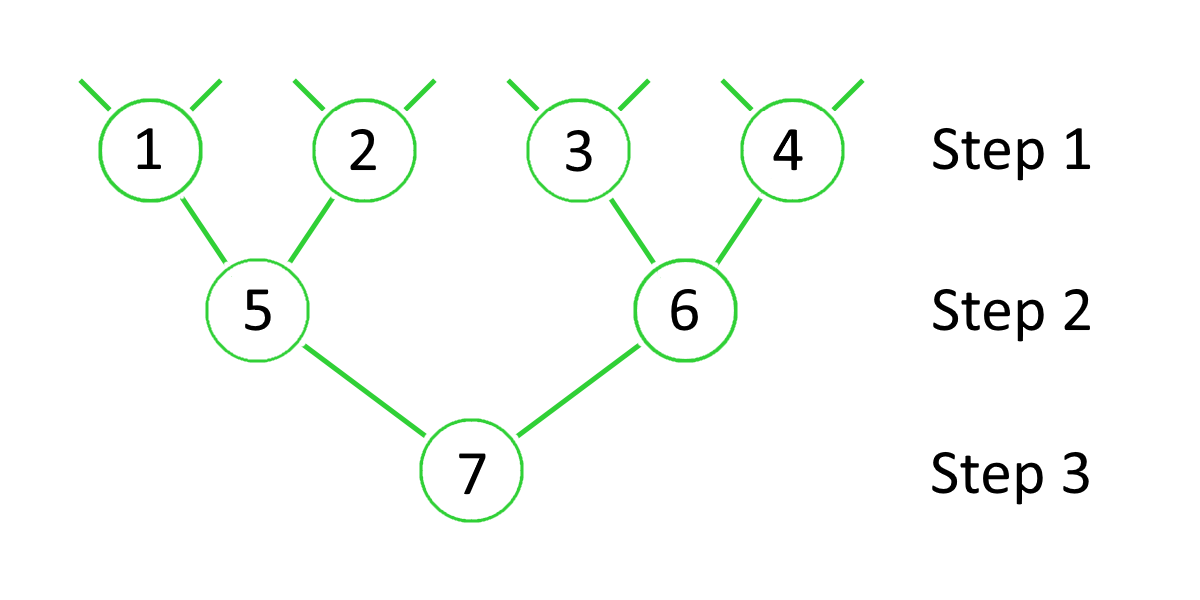
\includegraphics[width=0.6\textwidth]{figs/intro/step_work.png}
	}
	\caption{Step and work complexity example.}
	\label{fig:stepnwork}
\end{figure}

Step and work complexity is important in parallel programming, as we for a given algorithm, attempt to reduce the step complexity, thereby performing doing more in parallel at each step, by sacrificing work complexity. The idea behind this is that if the number of steps is reduced in our parallel implementation compared to our serial implementation, and work complexity is only slightly increased, our parallel algorithm will perform better then the serial algorithm.

	\section{Latency vs Bandwidth}
	\label{sec-lat-vs-band}
	So what exactly is the goal of parallelizing work? This can be described in terms of latency and bandwidth. For a regular serial algorithm, when increasing performance, we will see a latency decrease. Latency in this case will be the time between giving our algorithm a stimulus until it returns a response. For algorithms discussed in this course stimulus will be data, and thereby the time it takes for an algorithm to be applied to some data. For most serial algorithms, to lower latency, the amount of data it is performed on will have to be decreased. Most current CPU's are still built to be optimized for latency, where a fast response is wanted for some calculation.\\
This differs greatly from what is the goal of parallelizing work. Here the goal is to maximize the throughput, thereby maximizing how must data we can perform our algorithm on in a given time span. This means that we are willing to sacrifice latency on any given calculation, if it improve the calculations performed over time. This relates to the before mentioned step and work complexity, where, if the step complexity is reduced, and the work complexity/latency is only slightly increased, the throughput of an algorithm can be increased.

	\section{Approach to Parallelizing Code}
	\label{sec-app-to-par}
	So how does one approach parallelizing code or an algorithm, a systematic approach is called APOD which is an acronym for \texttt{Analyze}, \texttt{Parallelize}, \texttt{Optimize}, \texttt{Deploy}. APOD integrates software engineering principles, where an agile and iterative approach is taken to parallelize and optimize a program.\\
Each of these steps should be done individually, so given a problem, the first step is to \texttt{analyze}. The important part of the analyzation step is to first analyze to find out, what can be improved, where are the bottlenecks, how much can it be improved and is it worth the time to improve it.\
These are important, as they identify the critical sections in our program, with which we can then proceed to the next step \texttt{Parallelize}. in the parallelize step, the goal is to determine what approach can be taken to improve our problem. This could be choosing a library, picking an algorithm and/or programming the code. It is specifically important here that the right algorithm(s) for the task is chosen.\\
For the next step \texttt{Optimization}, the goal is as the name indicated to improve the program at hands. Primarily the focus here is on profile-driven optimization. It was described in \cref{sec-lat-vs-band} that with CUDA programming the goal is to improve throughput, which aligns with profile-driven optimization in that it is often possible to retrieve a measure on throughput, which can be used to compare whether optimization of the program actually improved throughput.\\
The final step \texttt{Deploy} is important because we want to test whenever improvement was beneficial to the "real" program. Does the solution achieved, solve our problem? did it help at all?\\ These questions are the reason why it is important that APOD is an iterative approach as if the answer was not to whether the problem was solved, a new round of APOD can be done, starting over with the \texttt{Analyse} step, again identifying bottlenecks. 
	

\chapter{GPU Hardware Architecture}
\label{ch-hw-gpu-hardware-architecture}
Modern software programmers have been using standard processing unit architectures, such as Central Processing Units (CPUs) for decades, where highly developed compilers help utilizing the underlying hardware.
However, Graphical Processing Unit (GPU) programmers must have considerable knowledge of the underlying hardware architecture to fully achieve optimized and efficient performance results.
Achieving such knowledge can be difficult as GPU hardware architecture is complex and comes in many variations.
This is a result of the major development of which GPUs has been undergoing, from the first GPUs emerging back in the late 1990s to the newest upcoming architectures not yet released.

The following sections will provide a understanding of how GPU hardware architecture is structured and how it works.
The first section briefly describes the early evolution of GPUs, leading to the birth of the GPUs used today, also defined as General Purpose Graphical Processing Unit (GPGPUs).
Hereafter, a type of GPGPU, namely the CUDA GPU hardware architecture is described in details, including its memory model.
Lastly, alternative GPU hardware architectures is presented, in addition with a description of 
the future architectures not yet launched.



 

	\section{Early Evolution}
	\label{sec-hw-early-evolution}
	The first GPUs  emerged back at the late 1990s, where a high demand of GPU accelerated 3D graphics served as the motivation for these new devices.
This demand for 3D graphics originated from the gaming industry \cite{Johansson2010}.
The GPU hardware architectures of these early versions was narrowly specialized.
Back then, the 3D rendering of the GPU, worked by having a fixed series of standard operations implemented in the hardware called fixed-function pipelines.
These functions were used to render 3D-scenes, and could for instance be to \textit{apply lightning}, or to \textit{add texture}.
Using a set of specialized hardware implementations to perform these operations, allowed for a large performance boost in comparison to the same execution handed out by the general purpose CPU.
However, using these fixed-function pipelines, meant that it was not possible to configure which function to perform, but only possible to adjust the parameters for these functions.
This limited the possibility for graphic programmers greatly, and led to a major switch in the GPU hardware architecture.

The first change to the architecture, was to remove the strictly fixed-function pipelines.
This was carried out by exchanging the highly specialized hardware functions with pools of flexible processor cores.
These pools are separated between processors responsible for pixel specific calculations (Pixel shading) and processors responsible for vertex specific calculations (Vertex shading) \cite{Johansson2010}.
The difference between these two shaders is that Pixel shaders operates per-pixel basis, and Vertex shaders perform operations to objects in a 3D environment.
Changing to flexible programmable processor cores, allowed developers to apply custom algorithms to the processing pipeline executed by the GPU.

However balancing the number of processors dedicated to either pixel or vertex calculations proved to be a difficult task.
As the workload to be distributed between the two depends on the individual application, a generic division of processors is unrealistic.
Usual applications contain a majority of pixels to be drawn in comparison to the amount of vertices to be calculated.
This distribution is however not alway true, as some applications demands for more verticies calculations than pixels.
This results in applications, where roughly half of the processing pool is idle for most of the processing time.
As this suboptimal uneven work distribution was unacceptable for a general purpose GPU, the architecture was further improved.

This led to the birth of the first GPGPU architecture. 
Here a narrowing from the two specialized processor types were unified to a single generic general purpose processor type, capable of handling the tasks of both of its predecessors.
This new processor is more complex, yet more flexible and allows for a efficient workload distribution as tasks are distributable throughout all processors.

The introduction of the new GPU hardware architecture containing a unified processor type started many research groups, with the focus of using the inherent computing power of GPUs for high-performance general purpose computing.
However, development of general purpose applications relied on programming frameworks used for graphical programming.
This forced programmers to transform their general computational problems to graphical problematics.
This demand led to GPGPU frameworks used today, such as NVIDIAs "CUDA" or AMDs "ATI Stream" \cite{Johansson2010}.
The NVIDIAs CUDA programming model is further described in \cref{ch-programming-model}, instead the remaining of this chapter will focus on the architectural part of the GPGPU.

	\section{CPU/GPU Architecture}
	\label{sec-hw-cpu-gpu-architecture}
	% https://www.youtube.com/watch?v=nRSxp5ZKwhQ - CUDA Part A: GPU Architecture Overview and CUDA Basics; Peter Messmer (NVIDIA)
% https://www.youtube.com/watch?v=lGefnd7Fmmo - Nvidia GPU Architecture
% https://www.slideshare.net/DhavalKaneria/gpu-with-cuda-architecture

% CPU:



% CPU/GPU:



% PCI Express:

\begin{figure}[ht]
	\centering
	\fbox{
		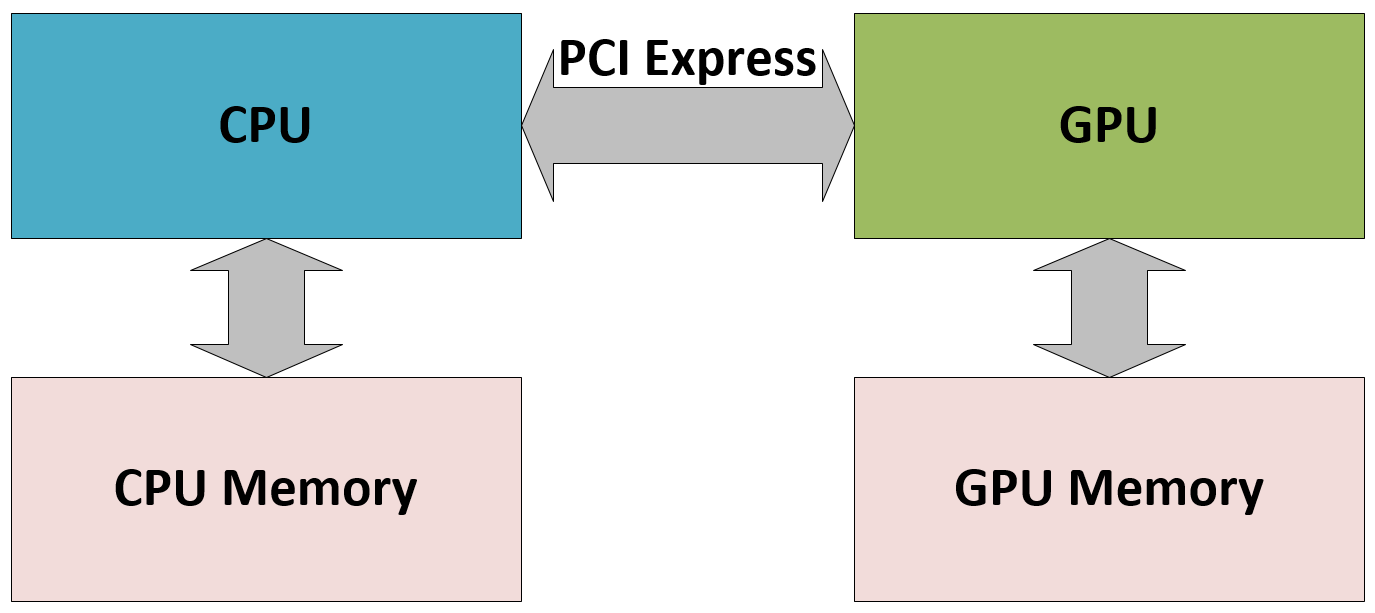
\includegraphics[width=0.8\textwidth]{figs/hw/hw-cpu-gpu}}
	\caption{TBD}
	\label{fig:hw-cpu-gpu}
\end{figure}




		
		\subsection{PCI Express}
		\label{sec:hw-pci-express}
		The communication between the CPU and GPU is handled through the high-speed serial computer expansion bus standard "Pheripheral Component Interconnect Express" more used in its abbreviation "PCI Express".

Devices connected by PCI Express communicate using a logical connection defined as a \textit{link}.
The link is a point-to-point channel, allowing both devices to send and receive PCI requests, such as configurations and memory read/writes.

A link is composed of 1, 2, 4, 8 or 16 \textit{lanes} \cite{wiki:pci}, which is furthermore composed of two differential signaling pairs, one pair for receiving data and the other for transmitting as presented on \cref{fig:hw-pci-express}.
Prior to PCI Express, the old PCI bus only allowed a single component to use the full bandwidth of the bus, as adding more devices would reduce the available bandwidth.
Lanes provide a guaranteed division of the bandwidth between all devices so that the amount of lanes used define the provided bandwidth.

\begin{figure}[ht]
	\centering
	\fbox{
		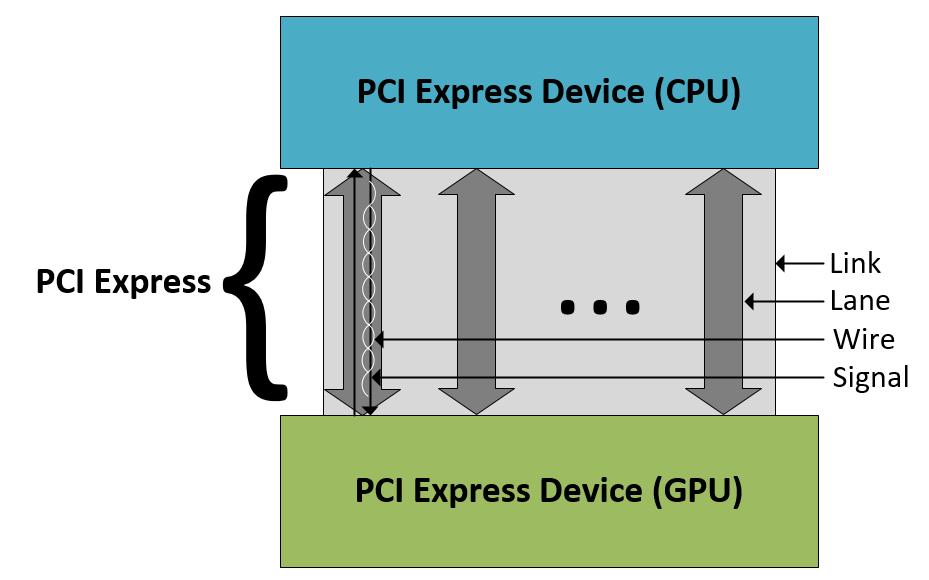
\includegraphics[width=0.8\textwidth]{figs/hw/hw-pci-express}}
	\caption{PCI Express link}
	\label{fig:hw-pci-express}
\end{figure}



As writing, PCI Express 3.x is the fastest bus version available, providing a bit rate up to 8GT/s (gigatransfers per second) equal to 985MB/s per lane.
As a single PCI Express 3.x slot can support up to 16 lanes, this results in a bit rate of up to 15.8GB/s.
The specifications for PCI Express 4.x and 5.x is however announced, with 4.x doubling the bit rate of 3.x to a total of 31.5GB/s for 16 lanes and 5.x expected to hit 63.0 or 49.2GB/s for 16 lanes \cite{wiki:pci}.

As mentioned lanes used in the bus are full-duplex, meaning that the upload speed to the GPU from the CPU is matched with the same download speed from the CPU to the GPU.
However, as the bandwidth is not cumulative, neither of the speeds will be doubled if the other is not transferring data.

PCI Express is a layered protocol, implementing layer 1, 2 and 4 of the OSI model, namely a \textit{physical layer},  a \textit{data link layer} and a \textit{transaction layer}.
% TODO: Consider extent: with OSI model
%https://web.archive.org/web/20140715120034/http://www.pcisig.com/developers/main/training_materials/get_document?doc_id=4e00a39acaa5c5a8ee44ebb07baba982e5972c67

	\section{GPU Architecture}
	\label{sec-hw-gpu-arhchitecture}
	As described in \cref{sec-hw-early-evolution}, the GPU hardware architecture has undergone a drastic development, and still is.
This section presents the GPU hardware architecture as a conceptual GPGPU architecture.
The architecture is presented from a GPU computing point of view, meaning that some elements which are only used by the GPU for graphical purposes are not included.

The GPU hardware architecture consists of three main block categories:
\begin{itemize}
	\item Streaming Multiprocessors (SMs)
	\item Streaming Processors (SPs) 
	\item Memory (Local, Shared \& Global)
\end{itemize}

On a high level, the GPU can be described as an array of \textit{N} SMs, each consisting of \textit{M} cores (SPs) as illustrated on \cref{fig:hw-gpu}. 
The number of SMs contained in GPUs varies a lot, from small GPUs only containing a single SM, to the newest Nvidia architecture \textit{Tesla V100} containing 84 SMs \cite{Nvidia2017}.
The number of SMs, and thereby the number of SPs, contained in the GPU enables more tasks to be processed at the same time or a single task to be processed faster if enough parallelism is implemented for this given task.
%TODO Tilføj evt. mere "general information" om GPU.


In addition to the three main block categories presented above, two other blocks is also presented on \cref{fig:hw-gpu}, namely the \textit{Host Interface} and the \textit{Global Scheduler}.

%Host Interface
The Host Interface is the logical representation of the GPUs PCI Express port.
It implements functionality needed to perform CPU/GPU interactions. 
The Host Interface does so, by reading commands such as \textit{copying memory} and  \textit{launching Kernels} (further described in \cref{sec-pm-kernels}), and dispatches these commands to the appropriate hardware units.
In addition to command handling, the Host Interface also facilitates synchronization between the CPU and GPU. 
For more information regarding the Host Interface, and the interactions between the CPU see \cite{Wilt2013} chapter 2.5 - CPU/GPU Interactions.

%Global Scheduler
The Global Scheduler, also known as "GigaThread Engine" by Nvidia \cite{Nvidia2009}, is responsible of distributing threads to SMs, where they are executed.
Scheduling is done by splitting threads into thread blocks, which are further described in \cref{sec-pm-kernels}.
After the threads are split into blocks, they are assigned to the SMs by the Global Scheduler.
The Global Scheduler has to take several hardware constraints into consideration.
First a single block cannot be split between two SMs.
Also, each SM is limited in the amount of threads and blocks that can be scheduled to it. 
More information regarding how threads and blocks are optimized split between SMs is covered in \cref{ch-opti-intro}.

\begin{figure}[ht]
	\centering
	\fbox{
		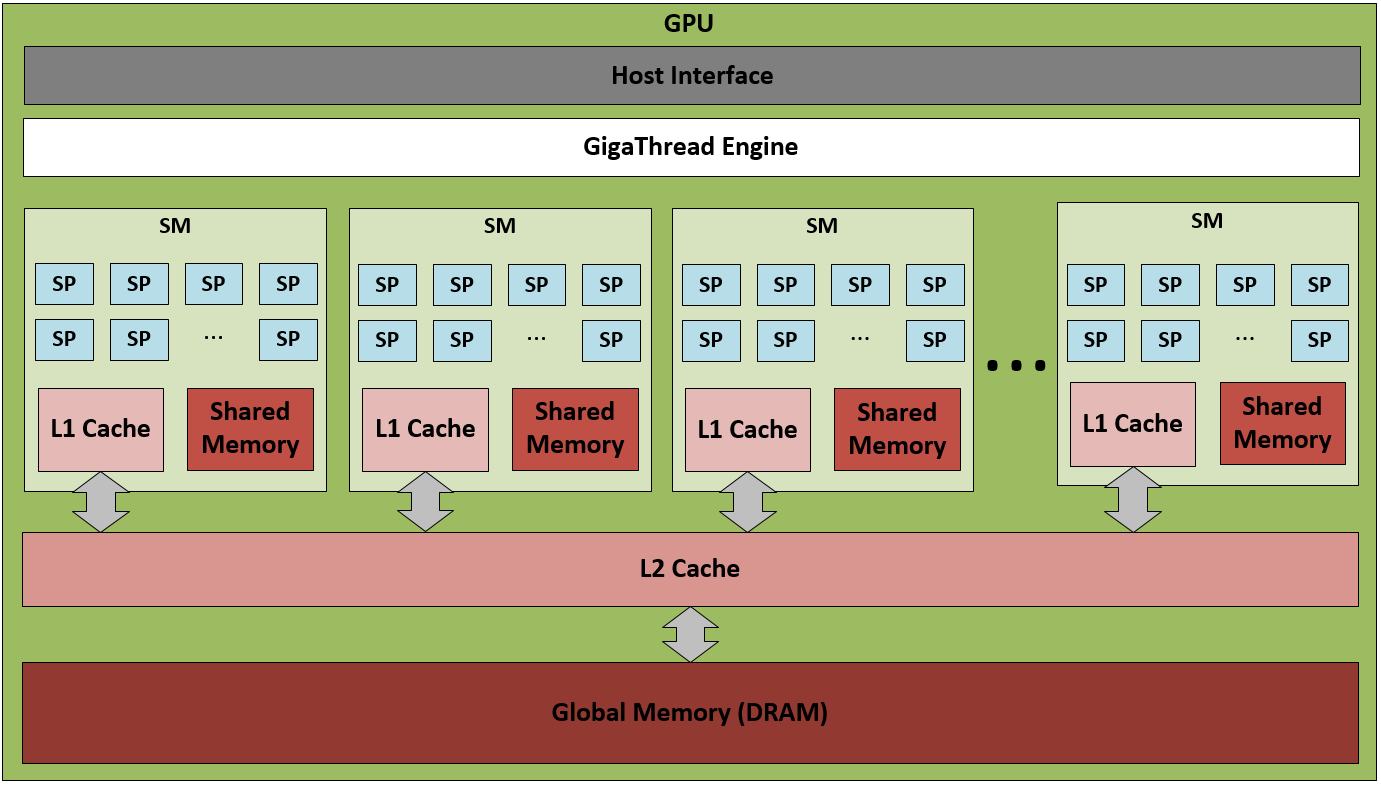
\includegraphics[width=1\textwidth]{figs/hw/hw-gpu}}
	\caption{Conceptual GPGPU hardware architecture}
	\label{fig:hw-gpu}
\end{figure}

Further information regarding SMs and SPs is covered in \cref{sec-hw-streaming-multiprocessors} and \cref{sec-hw-streaming-processors}.
Additional topics of the GPU hardware architecture is covered in the remaining subsections, including the memory model which is covered in \cref{sec-hw-memory-model}.
		
		\subsection{Streaming Multiprocessors}
		\label{sec-hw-streaming-multiprocessors}
		

\textit{Special Function Units (SFUs)} are a approximation units, which computes fast approximations of transcendental functions such as sine, cosine, reciprocal and square root.
%Each SFU also features four floating-point multipliers that can offer extra FP throughput in addition to SPs. The SFU pipelines are independent from the SP pipelines. 
% GPU Performance Modeling and Optimization cpt 6
% Add cite

\begin{figure}[H]
	\centering
	\fbox{
		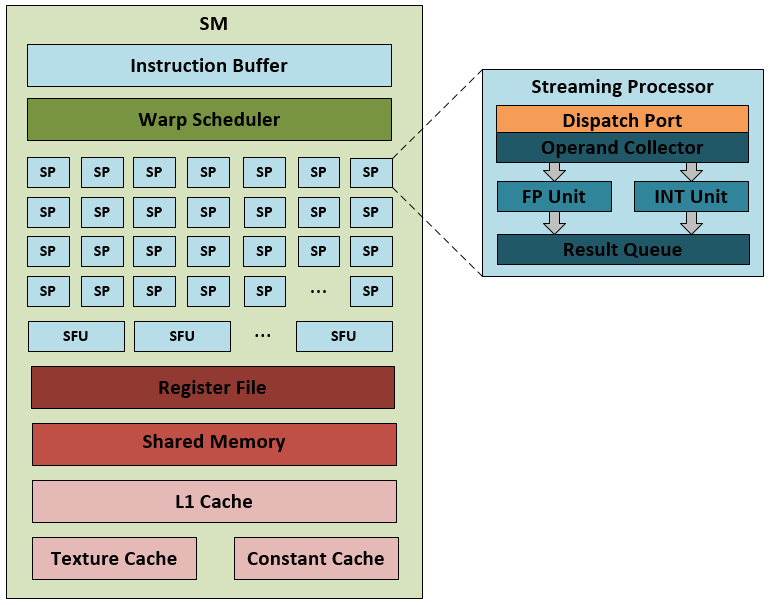
\includegraphics[width=1\textwidth]{figs/hw/hw-sm} }
	\caption{TBD}
	\label{fig:hw-sm}
\end{figure}
	
		\subsection{Streaming Processors}
		\label{sec-hw-streaming-processors}
		The Streaming Processors(SPs) goes under various different names including \textit{Scalar-Processors}, \textit{Execution Units} or the more famous \textit{CUDA Cores} by Nvidia.
SPs are the basic computing elements of a GPU, they perform fundamental operations, such as integer, floating-point, comparison and type conversions \cite{Li2016}.
SPs are comparable to the cores located in CPUs, containing similarities such as simultaneous multi-threading (SMT).
However, in order to increase the number of cores as seen for the GPU architecture, these SP cores need to be much simpler.
SPs are stripped from complex features normally resided in CPU cores such as:

\begin{itemize}
	\item \textbf{No Out-of-order execution,} which otherwise allows for parallel execution for the internal computational units within the core. 
	\item \textbf{No Cache memory,} instead the utilization of cache memory is moved to the SM. 
\end{itemize}

Furthermore, SPs does not contain its own computation registers, or instruction units.
Instead they depend on the Registration File and Warp Scheduler located in the SM.
Therefore SPs has to be considered as a part of a multi-processor to be compatible with the usual understanding of a computing core \cite{Maitre2013}.

By looking at the internal architecture of the SP, seen on \cref{fig:hw-sm}, it is seen that the SP contains five components:

\begin{itemize}
	\item \textbf{Dispatch Port -} The Dispatch Port is used to issue the execution of the given SP.
	\item \textbf{Operand Collector -} The Operand Collector is used to load operands from the Register File and then buffer them for computation in the SP.
	
	\item \textbf{FP Unit -} The Floating Point Unit is, by its name, used to perform floating point data instructions.
	It is one of the two dedicated data paths within the SP.
	Support of double-precision (64-bit) floating point units is handled different depending on the architecture version.
	Some architectures splits the double-precision instruction into multiple single-precision (32-bit) instructions, where other contain separate double-precision floating point units \cite{Johansson2010}.
	
	\item \textbf{INT Unit -} The Integer Unit, also known as Arithmetic Logic Unit (ALU), is the second data path within the SP. 
	As its name indicates, the INT Unit performs integer data operations.
	As the SP does not support Out-of-order execution, the two data paths cannot be active simultaneously.
	
	\item \textbf{Result Queue -} The Result Queue can be seen as the opposing component to the Operand Collector.
	It buffers output data from the FP Unit and the INT Unit, until it is written to the Register File.
	However, not all operations needs to be written back to the Register File.
	If the output of a operation is used as a intermediate result, which is to be consumed by another operation, it is possible to forward it directly to the other operation without saving it to the Register File.
	This concept is also known as a forwarding network, used in CPUs \cite{Kanter2009}.
\end{itemize}




		\subsection{Execution model - Warps \& Threads}
		\label{sec-hw-warps-threads}
		
% SIMT
This section covers the execution model of the GPU.
Based on Michael J. Flynn proposed Flynn's taxonomy \cite{Flynn1972}, used to identify computer architectures execution models, four categories were defined:

\begin{itemize}
	\item \textit{Single Instruction, Single Data} (SISD)
	\item \textit{Single Instruction, Multiple Data} (SIMD)
	\item \textit{Multiple Instruction, Single Data} (MISD)
	\item \textit{Multiple Instruction, Multiple Data} (MIMD)
\end{itemize}

The idea is to define how many instructions is performed on how much data.
For instance, SISD only allows for one instruction to be peformed on a single data input at a time, corresponding to a single-core CPU.
Based on SIMD, Nvidia introduced a new execution model \cite{Nvidia2009}, known as \textit{Single Instruction, Multiple Threads} (SIMT).
Now, lets see how this concept is mapped to the GPU architecture:


% Blocks -> Global Scheduler
A function running on the GPU is defined as a \textit{Kernel} (further descirbed in \cref{sec-pm-kernels}).
Once a Kernel is executed on the GPU, it is potentially handled by thousands of lightweighted threads running simultaneously.
As described in \cref{sec-hw-gpu-arhchitecture}, threads are grouped into \textit{thread blocks}, which are to be executed on SMs.
Once threads are divided into blocks, the blocks are dispatched by the Global Scheduler onto the SMs for execution.
A single SM can be assigned with multiple blocks, depending on the SMs limitations such as its memory.
In the case of multiple blocks assigned to a SM, the memory resources of the SM is divided evenly among the blocks.
\\\\
\textbf{Thread Assignment (Warps) -} Within the SM, the SIMT execution model is handled out by further organize the threads within the thread blocks into execution groups which is referenced to as SIMT units.
These SIMT units are better known as \textbf{Warps} using Nvidia terminology \cite{Nvidia2009} or Wavefronts by AMD \cite{Johansson2010}.
As the therm Warps is the mostly used, it is chosen for SIMT units throughout this report.
By the definition of the SIMT execution model, all threads within a warp is executed together, sharing the same instruction.
The main reason for grouping threads into warps, is to limit the amount of memory transactions performed by threads.
When threads have to access the Global Memory, the Warps are responsible for performing reads or writes for each thread within the warp, and in that way reduce the number of transactions performed.
The size of a warp is fixed to 32 threads/warp for all Nvidia GPU architectures \cite{Li2016}.
\\\\
\textbf{Thread Scheduling -} Scheduling of the warps is done by the Warp  Scheduler located within each SM.
As a warp is created, it is assigned to a warp scheduler, which it is assigned to for its remaining lifetime.
Each Warp Scheduler contains one or more Instruction Dispatch Units, which can be used to dispatch multiple different instructions at a time.
Depending on the architecture, the number of Warp Schedulers and Instruction Dispatch Units within a SM varies, however a conceptual example is used to illustrate how warp scheduling works.

\Cref{fig:hw-warp-scheduling} shows a scenario with a single Warp Scheduler, containing two Instruction Dispatch Units. 
In the example presented on the figure, the Warp Scheduler selects a warp, for instance the yellow marked Warp number 4 and splits it into two "half warps".
It hereafter executes two different Instruction to the two halfs, which are dispatched to execution on the SPs and/or SFUs.
However, this requires that the instructions handed out by the warps is executable by only half a warp.
Next, a new available warp is scheduled with a new set of instructions.
This rotation is continued until all instructions are executed.

\begin{figure}[ht]
	\centering
	\fbox{
		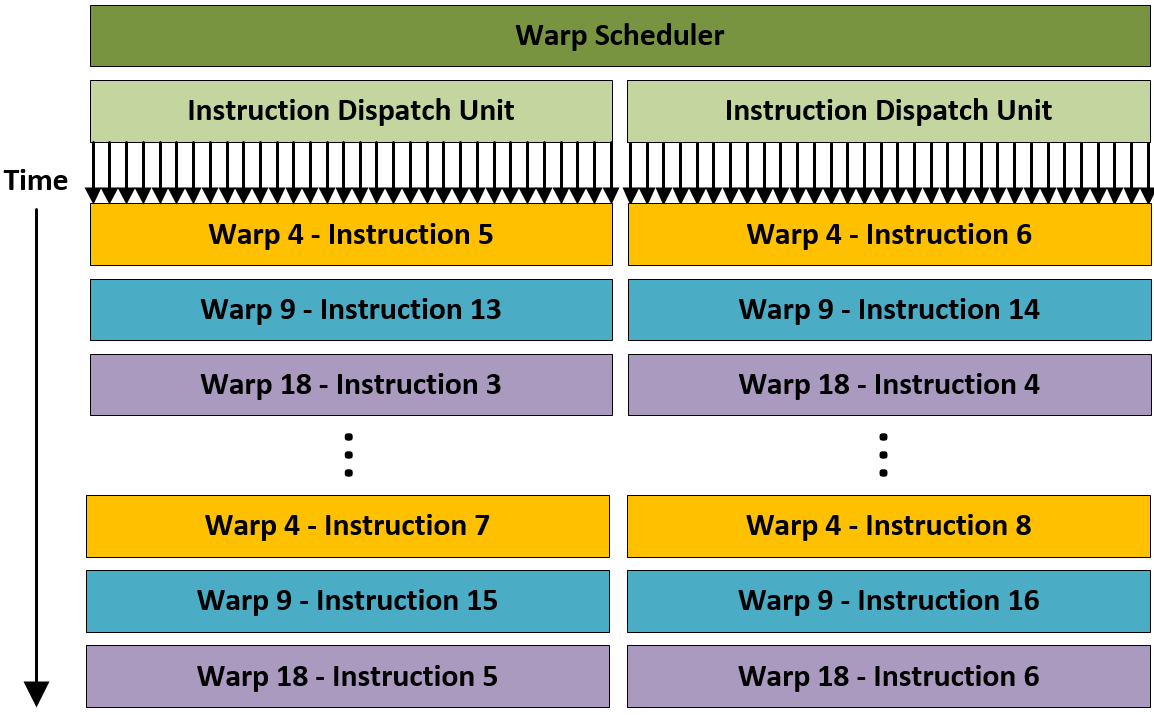
\includegraphics[width=0.8\textwidth]{figs/hw/hw-warp-scheduling}}
	\caption{Warp Scheduling}
	\label{fig:hw-warp-scheduling}
\end{figure}

Again, some architectures only contains one Instruction Dispatch Unit per Warp Scheduler, limiting the number of instructions that a warp can perform to one for all threads.

Prior to execution, instructions are located in a instruction queue, accessible to the Warp scheduler.
The warp scheduler is responsible of selecting the instructions that should be executed during the next clock cycle.
This selection is done based on two parameters, the status and priority of the instruction.

The status of an instruction is determined by its status flag, which can either be "ready" or "not ready".
When loaded into the instruction queue, an instructions flag is set to "not ready".
Once all operand and memory areas needed by the instruction is available, its status is changed to "ready".
The priority of an instruction is determined using a round-robin algorithm, which bases its decision on several different factors.

The instruction with the highest priority, and status flag set to "ready" is selected for execution by the Warp Scheduler.
\\\\
\textbf{Warp Divergence -} The SIMT execution model, however comes with a drawback.
In order to execute code where threads within the same warp is wished to perform different operations their SP cores have to diverge.
By diverge, it is meant that some cores are running instructions which they have in common, while others not having the same instructions remain idle and so on.
Such a code example could be a \textit{if-else} sentence as illustrated on
\autoref{lst:threaddiv} \& \cref{fig:hw-warp-div}.

\begin{lstlisting}[language=C,caption={Devergence generating code},label=lst:threaddiv]
if (threadId/2 == 0) {"Then"} 
else {"Else"}
\end{lstlisting}

 
\begin{figure}[ht]
	\centering
	\fbox{
		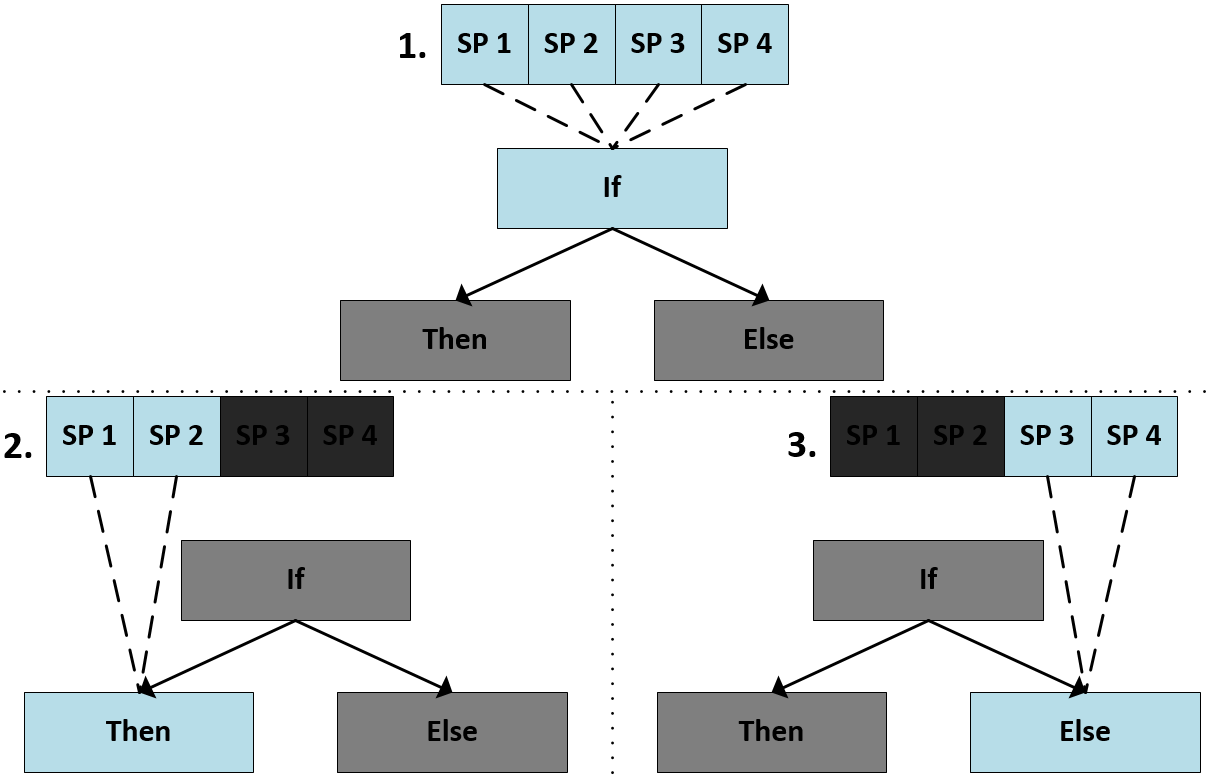
\includegraphics[width=0.7\textwidth]{figs/hw/hw-warp-div}}
	\caption{Warp Divergence}
	\label{fig:hw-warp-div}
\end{figure}

Here, first all threads test the \textit{if} condition.
Hereafter, threads running on SP1 \& SP2 executes the \textit{then} operation, while the other SPs remain idle.
Lastly, SP3 \& SP4 executes the \textit{else}, while SP1 \& SP2 idles.

This concept, defined as \textbf{Warp Divergence} obviously leads to performance losses, however \cref{ch-opti-intro} presents optimization aspects to this issue. 








		\subsection{Memory Model}
		\label{sec-hw-memory-model}
		%https://www.slideshare.net/maheshkha/cuda-tutorial (Memory space)
% https://www.slideshare.net/Hanibei/cuda-introduction - Kernel memory access



% https://www.microway.com/hpc-tech-tips/gpu-memory-types-performance-comparison/

%Husk at tjekke Shane Cook Hardware architecture afsnittet her.

%TODO Understanding NVIDIA GPGPU Hardware

%TODO Update to newest ( and consider all cahces)
\begin{figure}[H]
	\centering
	\fbox{
		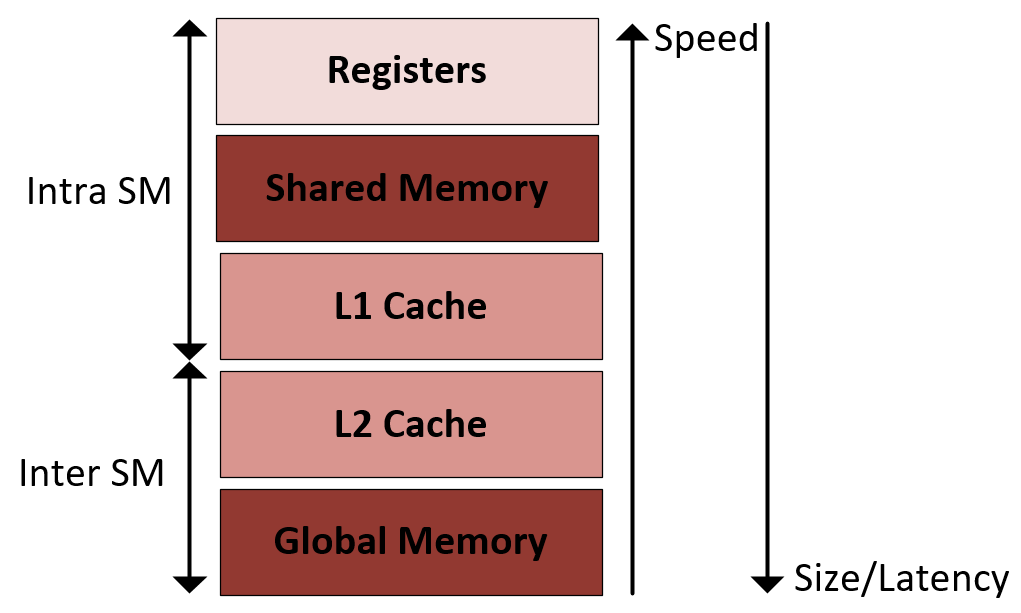
\includegraphics[width=0.6\textwidth]{figs/hw/hw-memory-schematic}}
	\caption{GPU memory schematic}
	\label{fig:hw-memory-schematic}
\end{figure}

\begin{figure}[H]
	\centering
	\fbox{
		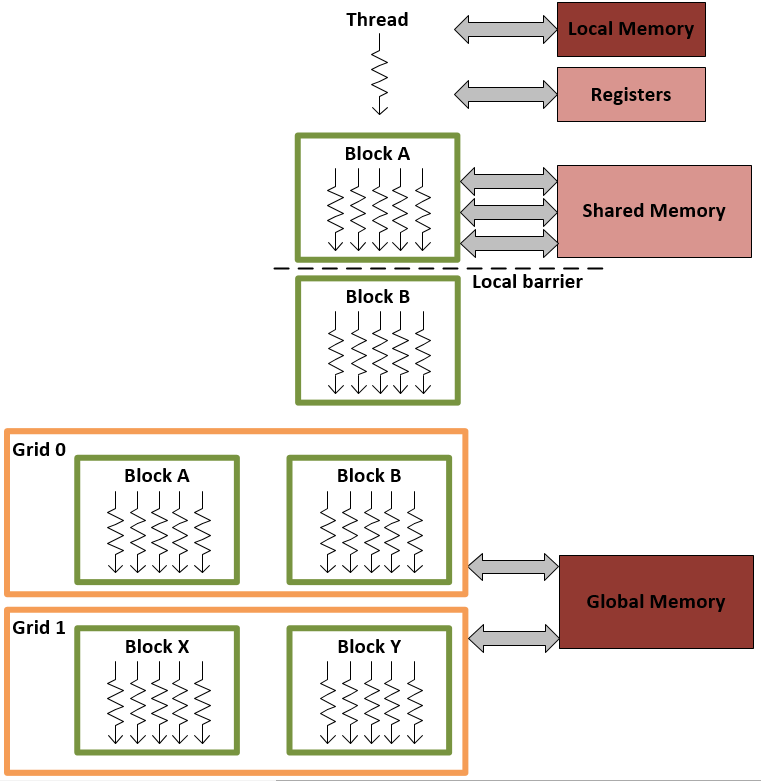
\includegraphics[width=0.8\textwidth]{figs/hw/hw-memory-model}}
	\caption{GPU memory model}
	\label{fig:hw-memory-model}
\end{figure}



	\section{GPU Variations}
	\label{sec-hw-variations}
	% Vis Warp scheduler eksempler


\chapter{\cuda{} Programming Model}
\label{ch-programming-model}
The \cuda{} programming model, is a heterogeneous model where both the CPU and the GPU are used.
In this context \textit{host} refers to the CPU and \textit{device} refers to the GPU and their respective memory.
The code run on the host also manages memory on the device and launches \textit{kernels} to be executed on the device.
The host and device are physically separated, which means that the host execution can run in parallel with the kernel execution on the device.
Kernels can briefly be described as functionality being executed by multiple threads in parallel on the device.

\noindent A typical sequence of operations performed in the \cuda{} programming model is as follows:
\begin{enumerateSmall}
	\item Allocate and initialize host and device memory
	\item Transfer data from host to device
	\item Execute kernel(s) on the device
	\item Transfer result(s) from device to host
\end{enumerateSmall}
The operations involved is described in details in the following sections.
The \cuda{} examples are written in "\cuda{} C", which is an extension to ANSI C, but the principles are generic and can be applied in all \cuda{} programming languages.
% mapping: Programming to Hardware

	\section{Kernels}
	\label{sec-pm-kernels}
	A kernel specifies functionality to be executed on a device.
It is specified using the declaration specifier \textit{\_\_global\_\_}, so that it can be distinguished from a regular C function.
When a kernel is launched, it is executed \textit{N} times in parallel by \textit{N} threads on the device.
The kernel is launched from the host, where it is specified how many \cuda{} threads to execute the kernel.
The launch of a kernel is specified by "$kernel\_name<<< number\_of\_blocks, number\_of\_threads\_in\_each\_block >>>$"
An example of a kernel and how it is being launched can be seen in \autoref{lst:kernel}.
\begin{lstlisting}[language=C,caption={Kernel example},label=lst:kernel]
__global__ void hello_world(float * d_out, float * d_in){
	print('hello world') }
int main(int argc, char ** argv) {
	hello_world<<<1, 100>>>(d_out, d_in); }
\end{lstlisting}
The kernel is launched with a single thread block with 100 threads.

	\section{Threads}
	\label{sec-pm-threads}
	A \cuda{} thread can be thought of as a lightweight thread, compared to a normal CPU thread.
It basically has access to the same resources but in a smaller scale.
As a kernel is executed in parallel by multiple threads, there must be a way to distinguish each thread from one another, so that they can perform different work.
Each thread is therefore given a \textit{thread index}, which can be accessed by each thread when executing a kernel.
It is syntactically done by accessing the struct \textit{threadIdx}, which contains the thread id in 3 dimension (x,y,z).
A simple example can be seen in \autoref{lst:threadIdx}.
\begin{lstlisting}[language=C,caption={Thread index example},label=lst:threadIdx]
__global__ void thread_idx_example(float* d_out, float* d_in){
	int idx = threadIdx.x;
	int idy = threadIdx.y;
	int idz = threadIdx.z; }
\end{lstlisting}
When a kernel is launched, the number of thread blocks (grid dimension) and the number of threads in a block (block dimension) must be specified.
The thread blocks are organized into a grid of blocks, in up to three dimensions (x,y,z).
In the same way, each block within the grid is comprised of multiple threads, also in up to three dimensions.
The thread hierarchy can be seen in \autoref{fig:grid-of-thread-blocks}, where the numbering is shown in "(x,y)" (z is zero in the example).
The grid dimension can be accessed by the struct \textit{gridDim}, The block id within the grid by \textit{blockIdx}, the block dimension by \textit{blockDim} and the thread id within a block by \textit{threadId}.
\begin{figure}[ht]
	\centering
	\fbox{
		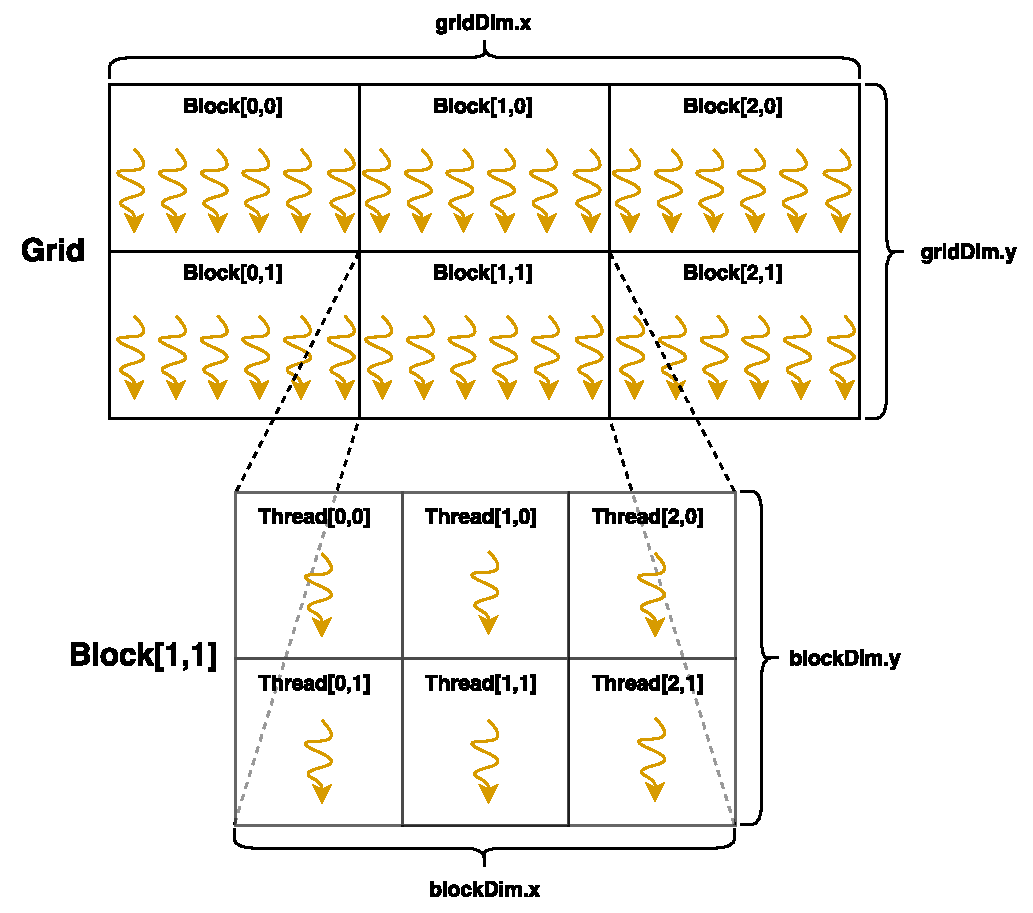
\includegraphics[width=0.6\textwidth]{figs/programming-model/grid-of-thread-blocks.pdf}
	}
	\caption{Grid of thread blocks}
	\label{fig:grid-of-thread-blocks}
\end{figure}
The maximum number of threads in a block is dependent on the specific device hardware, and on a lot of the current GPU's it can contain up to 1024 threads\cite{cuda:programmingguide}.
In \autoref{lst:thread-dim} is an example given of how to "create" a global thread id within the entire grid, so that each thread can perform independent work across thread blocks.
Another thing to notice is that to specify the size in three dimensions, the \textit{dim3} construct must be used.
\begin{lstlisting}[language=C,caption={Example of thread id usage in a grid of multiple thread blocks},label=lst:thread-dim]
__global__ void example(float * d_out, float * d_in){
	int myId = threadIdx.x + blockDim.x * blockIdx.x; }
int main(int argc, char ** argv) {
	dim3 blocks(x,y,z);
	dim3 threads(x,y,z);
	example<<<blocks, threads>>>(d_out, d_in); }
\end{lstlisting}
The number of blocks and threads to launch a kernel heavily depends on the specific application.
This is also valid in terms of the grid and block dimensions.
An example is that the dimensions can be chosen so that there is a natural mapping from a pixel in a picture, to each thread.
If the picture is black and white it would make sense to construct a 2D grid and if the picture contained RGB values, it would be preferable to construct a 3D grid.
So if the application contains multiple dimensions, it is possible to launch threads in multiple dimensions to ease the programming task.



	
	\section{Memory}
	\label{sec-pm-memory}
	+In relation to the \cuda{} programming model, memory are distinguished by \textit{host} and \textit{device} memory.
In \cuda{}, the host handles allocation of device memory as well as copying from host memory to device memory and visa versa.
An example can be seen in \autoref{lst:memory-host-to-device}, where device memory is allocated, host memory copied to device memory, a kernel is launched and memory is then copied back from device to host.
\begin{lstlisting}[language=C++,caption={Example of allocation and copying from host to device},label=lst:memory-host-to-device]
int main(int argc, char ** argv) {
	unsigned char *d_in;
	cudaMalloc( &d_in, numElems * sizeof(unsigned int) )
	cudaMemcpy(d_in, h_in, numElems * sizeof(unsigned int), cudaMemcpyHostToDevice)
	example<<<blocks, threads>>>(d_in);
	cudaMemcpy(h_in, d_in, numElems * sizeof(unsigned int), cudaMemcpyDeviceToHost) }
\end{lstlisting}
Inside a kernel, a thread can access different types of device memory (local, shared and global), as described in \autoref{mortens-memory-hierarchy}.
An example of accessing local and global memory can be seen in \autoref{lst:local-global-mem-acc}.
Local memory is everything allocated in the kernel, and can be thought of a variables allocated on the "stack". In the example, a local memory access is performed every time "myId" is accessed.
Global memory can be done by accessing raw device pointers passed to the kernel, as seen in the example by accessing "d\_out" and "d\_in".
The benefit of global memory is that it can be shared across thread blocks, but it is the slowest type of device memory.
\begin{lstlisting}[language=C,caption={Local and global memory access},label=lst:local-global-mem-acc]
__global__ void local_and_global_mem(float* d_out, float* d_in){
	int myId = threadIdx.x + blockDim.x * blockIdx.x;
	d_out[myId] = d_in[myId]; }
\end{lstlisting}
Shared memory is right in between local and global memory in terms of performance, but can only be accessed within a thread block.
An example of accessing shared memory can be seen in \autoref{lst:shared-mem-acc}.
When launching a kernel that uses shared memory, the number of bytes to allocate (per block) must be specified.
This can be done by using a third argument in the kernel launch, inside "$<<< >>>$".
In the kernel, the shared memory is declared by using the keyword and "\_\_shared" (and also "extern" as it can be accessed by multiple threads).
Each thread often copies global memory to shared memory and then accesses the shared memory as much as needed before copying back to global memory.
Before starting to use the shared memory it must be ensured that all threads have copied their value from global to shared memory.
This is ensured with the synchronizer "\_\_syncthreads" (explained in details in \autoref{sec-pm-synch}).
\begin{lstlisting}[language=C,caption={Kernel example},label=lst:shared-mem-acc]
__global__ void shared_mem(float * d_out, float * d_in){
	extern __shared__ unsigned int sdata[];
	int myId = threadIdx.x + blockDim.x * blockIdx.x;
	sdata[threadIdx.x] = d_in[myId];
	__syncthreads(); }
int main(int argc, char ** argv) {
	shared_mem<<< grid, threads, sizeof(unsigned int) * threads >>>( d_in, d_out ); }
\end{lstlisting}

%\autoref{fig:memory-hierarchy}
%\begin{figure}[ht]
%	\centering
%	\fbox{
%		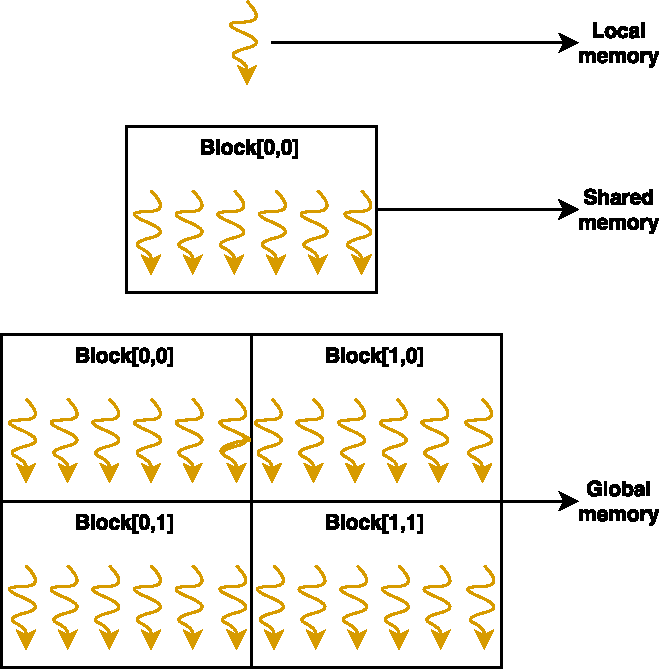
\includegraphics[width=0.6\textwidth]{figs/programming-model/memory-hierarchy.pdf}
%	}
%	\caption{Memory hierarchy}
%	\label{fig:memory-hierarchy}
%\end{figure}
	
	\section{Synchronization}
	\label{sec-pm-synch}
	syncthreads (only per block)
	
	\section{Streams}
	\label{sec-pm-streams}
	They way that the CPU communicates with the GPU is with commands.
This can for instance be memory transfers and kernel launches.
These commands are sent via streams, either implicitly or explicitly.
A stream is a virtual work queue (where the operations are executed in otder) used for asynchronous operations so that the CPU can operate concurrently with the GPU.
It is possible to have multiple streams and there can be a lot of reasons and benefits for this.
It is possible to perform memory copies concurrently with kernel executions.
To support this, the "copy engine" can perform a DMA transfer on the PCI-e bus while the SM's are executing a kernel.
Kernel launches are per definition asynchronous, but memory transfers can be either synchronous or asynchronous.
To make a memory transfer asynchronous, a different set of \cuda{} functions must be used (suffixed with a "Async").
An example of asynchronous kernel launches and memory transfers can be seen in \autoref{lst:stream-default-usage}.
As all the operations are asynchronous, they will simply be executed in the order, but the CPU will not wait for the operations to finish.
In this example no specific streams are linked to the operation, which means that all operations are linked to the default stream (number zero).
\begin{lstlisting}[language=C++,caption={Default stream usage},label=lst:stream-default-usage]
int main(int argc, char ** argv) {
	cudaMemcpyAsync( ... );
	example_kernel1<<< ... >>>
	cudaMemcpyAsync( ... )
	example_kernel2<<< ... >>> }
\end{lstlisting}
If one would like to use different streams, can be de declared and used as seen in \autoref{lst:stream-cre-des}.
From here, the entire life-cycle of a \cuda{} stream can be seen.
The stream is simply used by passing the \cuda{} struct to the async memory transfer function and the kernel launch.
\begin{lstlisting}[language=C++,caption={Stream creation, usage and destruction},label=lst:stream-cre-des]
int main(int argc, char ** argv) {
	cudaStream_t stream;
	cudaStreamCreate(&stream);
	cudaMemcpyAsync(d_in, h_in, 10 * sizeof(unsigned int), cudaMemcpyHostToDevice, stream);
	example_kernel<<<10, 1024, 0, stream>>>(d_in, 10)
	cudaStreamDestroy(stream) }
\end{lstlisting}
Using streams are for instance beneficial if you have to perform computations on a large amount of data that are bigger than the GPU memory.
There are different ways to do this, where two scenarios are described below and visualized in \autoref{fig:streams-advantage}.
\begin{enumerate}
	\item[\textbf{Scenario 1}]
		\begin{enumerate}
			\item Splitting the data into smaller chunks that fit in GPU memory
			\item Copy chunk from CPU to GPU
			\item Process data
			\item Copy processed data back to the CPU
		\end{enumerate}
	\item[\textbf{Scenario 2}]
			\begin{enumerate}
				\item Splitting the data into chunks half the size of scenario 1
				\item Copy chunk from CPU to GPU to fill half of GPU memory
				\item Process data and concurrently copy new chuck of data to GPU (GPU memory is now full)
				\item Copy processed data back to the CPU and concurrently copy new chuck to GPU (replacement of the processed data)
		\end{enumerate}
\end{enumerate}
\begin{figure}[ht]
	\centering
	\fbox{
		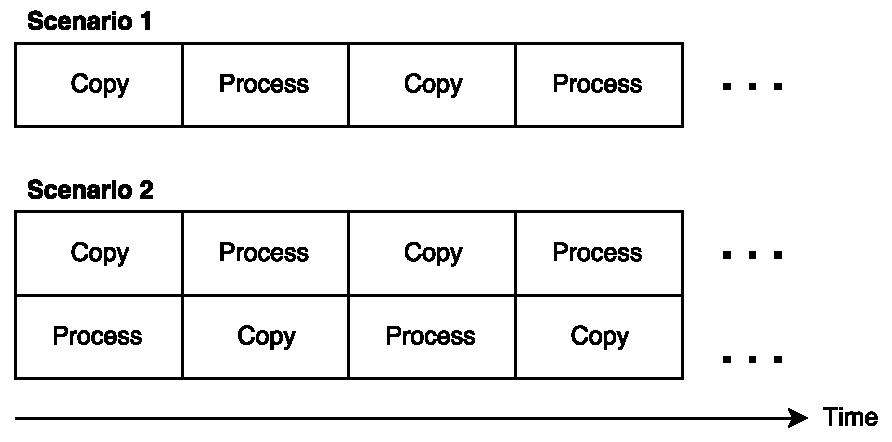
\includegraphics[width=0.5\textwidth]{figs/programming-model/streams.pdf}
	}
	\caption{Advantage of using streams}
	\label{fig:streams-advantage}
\end{figure}
To sum up, it can generally be be advantageous to use stream to overlap memory and computation and help fill GPU with smaller kernels.
%caveats --> streams and events	
	
	\section{Error Checking}
	\label{sec-pm-error-checkng}
	In \cuda{} all synchronous operations returns an error code.
This error code can be checked with \textit{cudaPeekAtLastError()} or \textit{cudaGetLastError()}.
It is a different story for asynchronous functions, as these cannot return the error code immediately, because they have not finished its execution when the function returns.
The only way to retrieve the error code is to call \textit{cudaDeviceSynchronize()} right after the asynchronous function call.
This functions waits for the asynchronous call to finish and afterwards is it possible to retrieve the error code in the same way as for synchronous function calls.
The use of error checking can be beneficial during the development of \cuda{} programs to explicitly check if any errors occur \cite{cuda:programmingguide}. 
 
	
	\section{Dynamic Parallelism}
	\label{sec-pm-dynamic}
	Dynamic parallelism is a "relative" new feature in the \cuda{} programming model.
It was added in \cuda{} 5.0 and it allows kernels to launch other kernels i.e threads can launch more threads.
An example of nested parallelism can be seen in \autoref{fig:nested-kernel} (The letters symbolizes kernels inside a \cuda{} stream).
Kernels A,B and C are launched by the host (Parent)
When kernel B executes, it launches kernels D, E and F (Children) and when kernel E executes, it launches G,H and I (Grand children).
\begin{figure}[ht]
	\centering
	\fbox{
		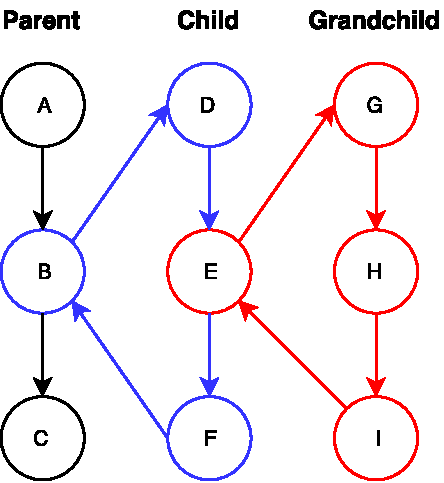
\includegraphics[width=0.3\textwidth]{figs/programming-model/recursive-kernel.pdf}
	}
	\caption{Nested kernel call}
	\label{fig:nested-kernel}
\end{figure}
The feature was added to express nested and recursive parallelism more easily, as this type of parallelism arises naturally in many applications.
An example is quick sort which is a "divide and conquer" algorithm which is well suited for recursion.
The idea is that an element is picked (called a pivot point), and all elements less that this point is reordered to come before the pivot point, and all points larger to come after.
This is performed recursively until all elements have been sorted.
An example can be seen in \autoref{fig:recursion-quicksort}
\begin{figure}[ht]
	\centering
	\fbox{
		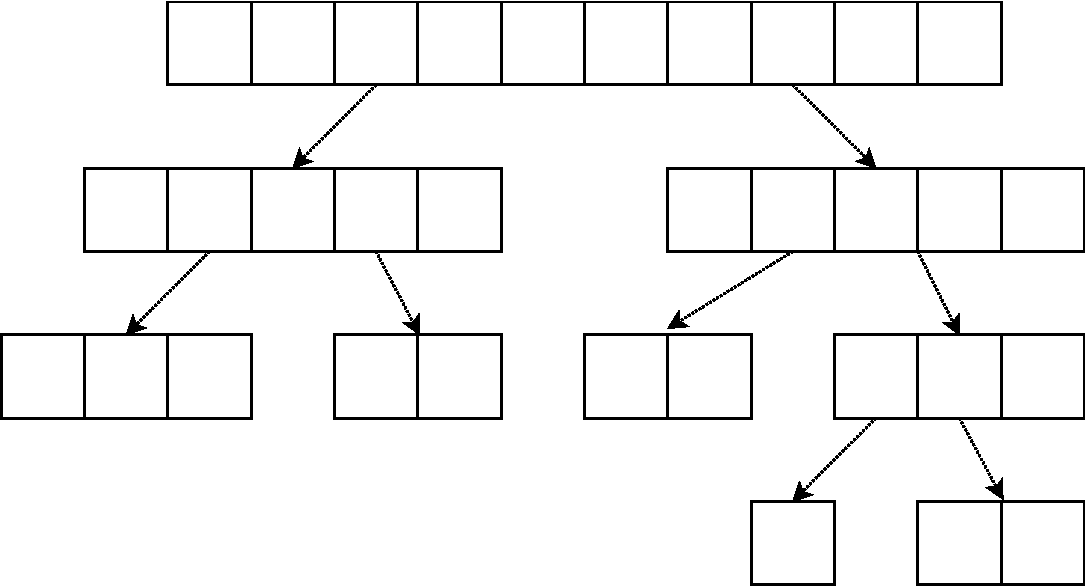
\includegraphics[width=0.4\textwidth]{figs/programming-model/recursion-quicksort.pdf}
	}
	\caption{Recursion and quicksort}
	\label{fig:recursion-quicksort}
\end{figure}

Launching kernels from within other kernels can be beneficial in some applications, but there are also things to watch out for when using this technique in \cuda{}.
Shared memory cannot be passed to a child kernel, so there is a performance penalty in having to copy data to global memory.
One should also be aware that every thread is executing the same program/kernel, which means that every thread will launch child kernels.
	
	\section{How to Compile and Run a \cuda{} Program}
	\label{sec-pm-compile-run}
	Kernel code can be written directly using the CUDA instruction set called PTX, but it is usually more beneficial to use a higher level language such as C.
Both of them must be compiled into machine code before it can be used.
This can be done by the Nvidia CUDA Compiler (NVCC).
As \cuda{} code runs on both host and device, NVCC separates the two, and sends the CPU code to a C compiler (GCC for instance) and the device code is further compiled to PTX instructions by NVCC \cite{cuda:programmingguide}.
At the end, the PTX and CPU (assembly) instructions are compiled to machine code which can be transferred to the host and device to be executed.
The flow is depicted in \autoref{fig:nvcc-compiler}
\begin{figure}[ht]
	\centering
	\fbox{
		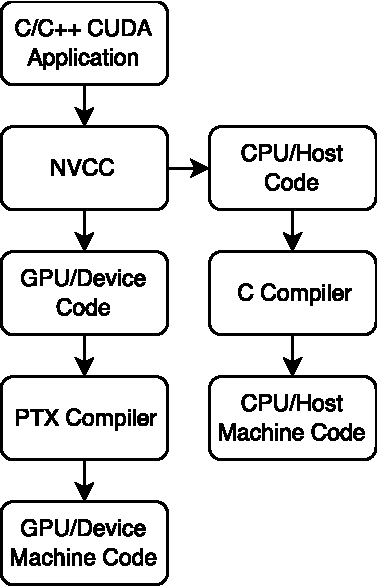
\includegraphics[width=0.3\textwidth]{figs/programming-model/NVCC.pdf}
	}
	\caption{NVCC compiling}
	\label{fig:nvcc-compiler}
\end{figure}
To separate C/C++ code files from \cuda{} code files, \cuda{} uses the file extension ".cu".
A simple example of compiling and running a .cu file in Linux can be seen in \autoref{lst:compile-example}.
\begin{lstlisting}[language=bash,caption={Compilation and run example},label=lst:compile-example]
	nvcc -c helloworld.cu -o helloworld
	./helloworld 
\end{lstlisting}
This is only valid for very simple cuda programs, as there are a lot of different compiler flags to be used, depending on the platform etc.


\chapter{Parallel Communication Patterns}
\label{ch-patterns}
In parallel computing tasks (threads) need to work together to solve a given problem. 
To be able to solve a problem the different tasks need to communicate with each other.
There are different parallel communications patterns such as map, transpose, gather and stencil.
Such communication patterns are essential for implementing more complex parallel algorithms.
	
	\section{Map}
	\label{sec-map}
	In the map communication pattern each tasks reads and writes to specific data elements in memory.
In its simplicity, the same function or computation is done on each piece of data as seen in bla. bla.

---add fig here

In the this way there is a one-to-one correspondence between the input and output.

This corresponds to that one thread will be doing each task in CUDA.
An example is seen listing bla. bla.

---add code

Here the kernel is launched in one block which spawns 64 threads and each thread does the same computation which is to square its thread id.
	
	\section{Gather}
	\label{sec-gather}
	The gather communication pattern gathers input data elements together from different places in memory and computes a single output result.
This is different from the map pattern since this pattern maps multiple inputs to a single output.
In this way the gather pattern has a many-to-one correspondence between inputs and outputs as can be seen in \autoref{fig:gather}.

\begin{figure}[ht]
	\centering
	\fbox{
		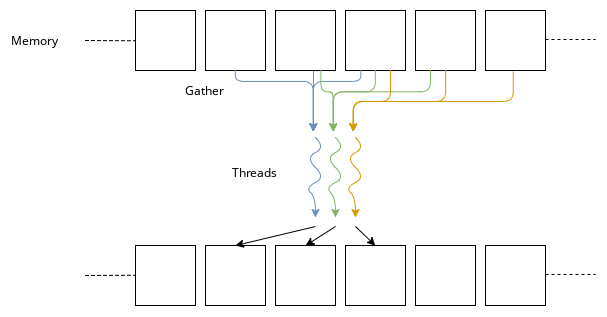
\includegraphics[width=0.75\textwidth]{figs/parallelgather.png}
	}
	\caption{Gather Pattern}
	\label{fig:gather}
\end{figure}

This parallel communication pattern can for instance be applied to image processing applications such as implementing blurring, sharpening, edge detection and more on an image.
This is done by 'sliding' a \textit{kernel} \footnote{Sometimes also called a \textit{convolutional matrix} or \textit{mask}} over the entire image to get a new image with a desired effect.
The effect which is applied to the new image is determined by the values in the kernel, but the parallel pattern which is used to implement this is the same, namely the gather pattern.
An example of applying a kernel to an image is seen in \autoref{fig:kernel}.
\begin{figure}[ht]
	\centering
	\fbox{
		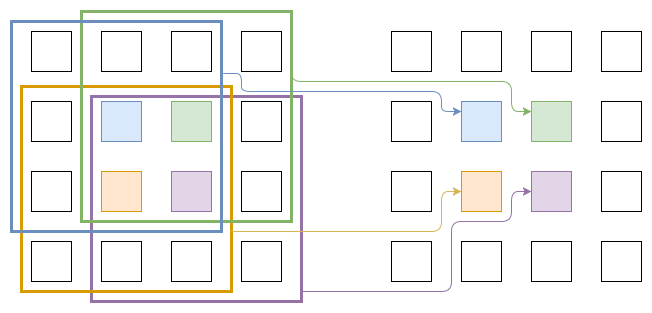
\includegraphics[width=0.6\textwidth]{figs/parallelblur2.png}
	}
	\caption{Example of a kernel operation}
	\label{fig:kernel}
\end{figure}
Using such a parallel communication pattern can vastly improve the computation time of applying for instance a kernel to an image.
Say that with a kernel with $\mathtt{NxN}$ dimensions and an image with $\mathtt{K}$ pixels the running time would be $\mathtt{O(N\cdot K)}$ on serial processor compared to $\mathtt{O(N)}$ in parallel, assuming that $K$ threads can be spawned on the GPU.

%TODO: make small code example of gather
	
	\section{Scatter}
	\label{sec-scatter}
	The scatter communication pattern reorganizes data and writes a single input data element to a single or multiple different output element(s) in memory.
This communication is used when a parallel tasks needs to write its result to a specific or multiple output elements.
It is similar to gather but instead it has a one-to-one/one-to-many correspondence between input and output(s) as seen in \autoref{fig:scatter}.
\begin{figure}[ht]
	\centering
	\fbox{
		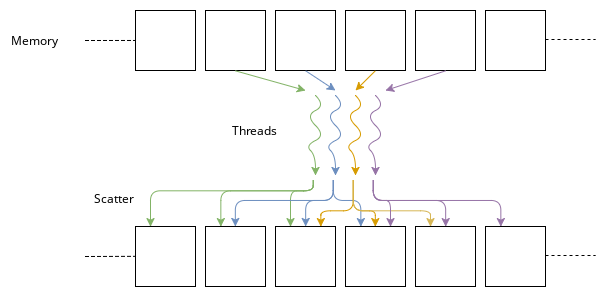
\includegraphics[width=0.6\textwidth]{figs/patterns/parallelscatter.png}
	}
	\caption{Scatter Pattern}
	\label{fig:scatter}
\end{figure}
\autoref{fig:scatter} suggests that there might be a synchronization issue which could lead to a \textit{data race}.
The problem is that several threads will very likely try to write to the same place in memory.
Say for instance that each thread has to increment a variable in memory which can be accessed by any thread.
This increment might not be correct because the variable might have been updated by another thread \textit{after} the variable has been read, which leads to data inconsistency.
This can be avoided by synchronizing threads or declaring the memory section as atomic.

The scatter pattern can for instance be used in combination with the gather pattern for representing sparse matrices which is more thoroughly described in section ?? bla. bla.

	
	\section{Stencil}
	\label{sec-stencil}
	The stencil communication pattern is a special case of the gather pattern.
The stencil pattern reads multiple elements in memory defined by some specific offset or pattern to a given input.
This offset or pattern defines specific characteristics of a stencil.
Examples of specific stencils are \textbf{2D/3D von Neumann} and \textbf{2D/3D Moore}.
For further figure references in this section, the green cube/square symbolizes the input element of a stencil operation.
\\\\
The 2D \textbf{von Neumann stencil} reads the input, top, bottom, left and right elements relative to the input element in an array.
The number of \textit{N} elements that are read in a von Neumann stencil in each direction is determined by a "\textit{N}-point von Neumann stencil".
This means that for a 5-point 2D von Neumann stencil would in total result in five reads, while a 9-point 2D von Neumann stencil would in total result in 9 reads.
The number of \textit{N} points in a 2D von Neumann stencil can be formalized as $(N\bmod 4)=1\equiv true$.
Examples of different 2D von Neumann stencils are seen in \autoref{fig:2DvonNeu}.
\begin{figure}[ht]
	\centering
	\begin{subfigure}{.33\textwidth}
		\centering
		\fbox{
			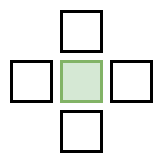
\includegraphics[width=0.4\textwidth]{figs/patterns/5point2DvonNeu.png}
		}
		\caption{5-point 2D von Neumann stencil}
		\label{fig:5p2DNeu}
	\end{subfigure}%
	\begin{subfigure}{.33\textwidth}
		\centering
		\fbox{
			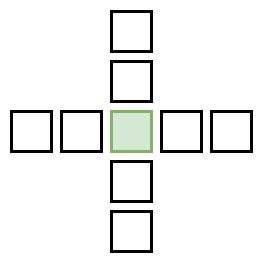
\includegraphics[width=0.6\textwidth]{figs/patterns/9point2DvonNeu.png}
		}
		\caption{9-point 2D von Neumann stencil}
		\label{fig:9p2DNeu}
	\end{subfigure}
	\begin{subfigure}{.33\textwidth}
		\centering
		\fbox{
			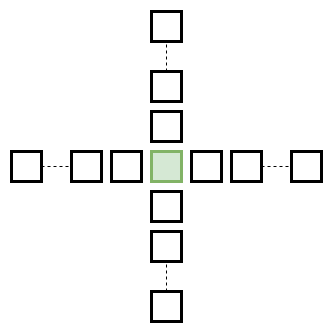
\includegraphics[width=0.6\textwidth]{figs/patterns/Npoint2DvonNeu.png}
		}
		\caption{N-point 2D von Neumann stencil}
		\label{fig:Np2DNeu}
	\end{subfigure}%
	\caption{Different 2D von Neuman stencils}
	\label{fig:2DvonNeu}
\end{figure}
The von Neumann stencils generalizes also to three dimensions.
The main idea is the same as for 2D but with an added dimension.
The number of read data points is thus more compared to the 2D case, and the number of \textit{N} points in a 3D von Neumann stencil can be formalized as $(N\bmod 6)=1\equiv true$.
Examples of 3D von Neumann stencil is seen in \autoref{fig:3DvonNeu}.
\begin{figure}[ht]
	\centering
	\begin{subfigure}{.33\textwidth}
		\centering
		\fbox{
			
\includegraphics[width=0.4\textwidth]{figs/patterns/7point3DNeu.png}
		}
		\caption{7-point 3D von Neumann stencil}
		\label{fig:7p3DNeu}
	\end{subfigure}%
	\begin{subfigure}{.33\textwidth}
		\centering
		\fbox{
			
\includegraphics[width=0.6\textwidth]{figs/patterns/13point3DNeu.png}
		}
		\caption{13-point 3D von Neumann stencil}
		\label{fig:13p3DNeu}
	\end{subfigure}
	\begin{subfigure}{.33\textwidth}
		\centering
		\fbox{
			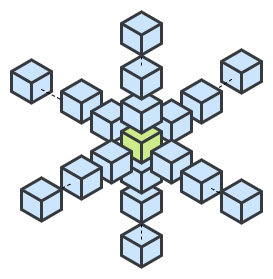
\includegraphics[width=0.6\textwidth]{figs/patterns/Npoint3DNeu.png}
		}
		\caption{N-point 3D von Neumann stencil}
		\label{fig:Np3DNeu}
	\end{subfigure}%
	\caption{Different 3D von Neuman stencils}
	\label{fig:3DvonNeu}
\end{figure}
\\\\
\textbf{Moore stencils} are almost the same as von Neumann stencils, with the exception that  they read \textit{all} neighbors relative to the input element.
This means that the shape of a 2D Moore stencil is a square, while the shape of a 3D Moore stencil is a cube.
The number of \textit{N} points in a 2D Moore stencil can be formalized as $(N\bmod 8)=1\equiv true$ and for the 3D case as $(N\bmod 26)=1\equiv true$.
Examples of Moore stencils is seen in \autoref{fig:Moore}.
\begin{figure}[ht]
	\centering
	\begin{subfigure}{.5\textwidth}
		\centering
		\fbox{
			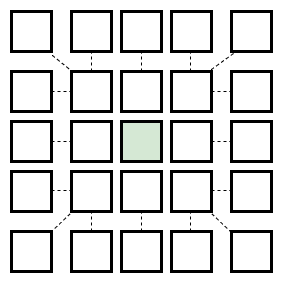
\includegraphics[width=0.4\textwidth]{figs/patterns/Np2dMoore.png}
		}
		\caption{N-point 2D Moore stencil}
		\label{fig:Np2DMoore}
	\end{subfigure}%
	\begin{subfigure}{.5\textwidth}
		\centering
		\fbox{
			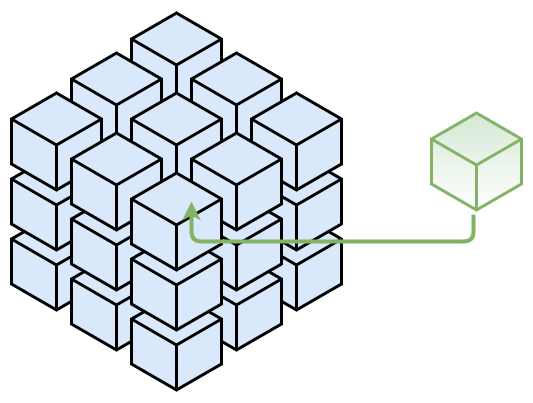
\includegraphics[width=0.6\textwidth]{figs/patterns/Np3dMoore.png}
		}
		\caption{27-point 3D Moore stencil}
		\label{fig:27p3DMoore}
	\end{subfigure}
	\caption{Different types of Moore stencils}
	\label{fig:Moore}
\end{figure}
As can be from \autoref{fig:27p3DMoore} the input element is surrounded by other other elements in the memory grid, and for this reason it is a bit difficult to illustrate that the input element resides inside the cube.
Notice that using 2D Moore stencils is a way of how kernels for image processing are implemented as described in \autoref{sec-gather}.
\\\\
An example of applying a 2D von Neumann stencil to an array of inputs is illustrated in \autoref{fig:2dMooreEx}.
In this case a thread is responsible for applying a single stencil to an input element.
\begin{figure}[ht]
	\centering
	\fbox{
		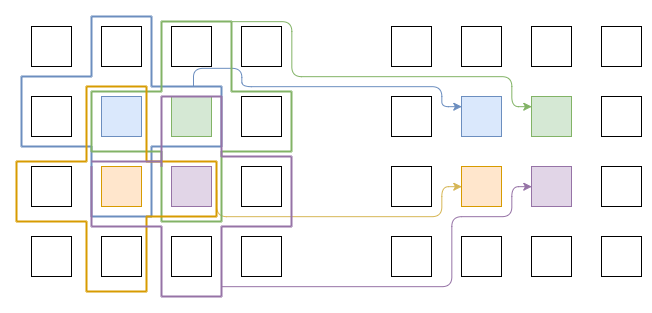
\includegraphics[width=0.6\textwidth]{figs/patterns/2dMooreEx.png}
	}
	\caption{Example of applying 2D Moore stencil}
	\label{fig:2dMooreEx}
\end{figure}
Implementing these stencils are done the same way as with the gather pattern, since stencils are special cases of this pattern.
In the case of applying stencils in parallel exploits a lot of data reuse since multiple threads are overlapping each other.
Implementing the stencil pattern maps very well to CUDA, since it is possible to represent both 2D and 3D structures in CUDA.
	
	\section{Transpose}
	\label{sec-transpose}
	The transpose communication pattern reorganizes a given data structure into its transpose representation.
Transpose is a special case of the scatter pattern since it writes its input into a different location in the output memory.

For example it might desirable to transpose a matrix which is represented by a 2D array, laid out in row-major order\footnote{Consecutive elements of a row reside next to each other}.
Transposing such a 2D array will lay out the matrix in column-major order in stead.
An example of transposing a 2D array using the scatter pattern is seen in \autoref{fig:transpose}.
Each thread reads an element from the array but writes its value somewhere scattered in memory according to its stride in the row column transpose.
In the example seen in \autoref{fig:transpose} the stride is three such that each input element with index $i$ will be scattered into "$i\bmod 3$" index in the output array.
\begin{figure}[ht]
	\centering
	\fbox{
		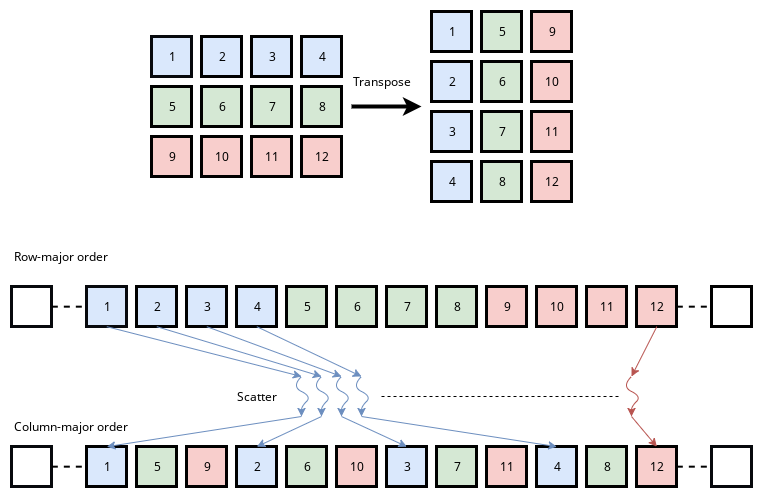
\includegraphics[width=0.6\textwidth]{figs/patterns/parallelTranspose.png}
	}
	\caption{Transpose Pattern}
	\label{fig:transpose}
\end{figure}
A major benefit for using the transpose pattern is that the input structure is reorganized into a more efficient memory structure since CUDA uses coalesced memory transactions when reading from and writing to memory.
The transpose pattern has many use case such as image processing, matrix algebra and more.
	
\chapter{Algorithms}
\label{ch:algorithms}
The idea behind the GPU is to have multiple threads working together, solving a common problem, in an efficient way. Parallel communication patterns can be used to solve a subset of parallel computation problems, but to solve larger similar problems, parallel algorithms are important. Algorithms use a defined number of steps or procedures to solve different types of problems. Many of the algorithms known from serial computation, may be inefficient or inadequate for parallelization, so it is important to know the only parallel algorithms. This section will describe and discuss some of the important algorithms for parallel programming including reduction, scan, histogram, sort, compact and allocate.   

	\section{Reduction}
	\label{sec:al_reduction}
	A highly used pattern in parallel computing is reduction. Reduction combines all elements in an array to a single element using an reduction operator. This can for example be used to calculate the sum or product of an array. In order for a reduction to work the reduction operator must be both binary and associative. Binary means that the operator is two-to-one, combining two element. Associative means that the order of which operations are performed does not effect the result, which can be mathematical expressed as \cref{def:reduce_associative}.

\begin{definition} 
\label{def:reduce_associative}
\textit{For an operator $\oplus$ to be associative the following statement must be true:}
\begin{center}
	$(a \oplus b) \oplus c = a \oplus (b \oplus c).$
\end{center}
\end{definition}

\noindent Addition and multiplication operators are associative while subtraction and division is not. The reduction can also be formally defined, which was done by Blelloch in \cite{BlellochTR90}, as seen in \cref{def:reduce}.

\begin{definition} 
	\label{def:reduce}
	\textit{The reduction operation takes a binary associative operator $\oplus$ with identity $\mathcal{I}$, and an ordered set}
	\begin{center}
		$[a_0, a_1,...,a_{n-1}]$ 
	\end{center}
	\textit{of $n$ elements, and returns the value}
	\begin{center}
		$a_0 \oplus a_1 \oplus ... \oplus a_{n-1}.$
	\end{center}
\end{definition}
\begin{example}
	\textit{For the binary associative operator $+$ and the ordered set}
	\begin{center}
		$[1,2,3,4,5,6,7,8]$ 
	\end{center}
	\textit{the return is}
	\begin{center}
		$36$
	\end{center}
	\end{example}

A visual representation of a serial reduction is seen on \cref{fig:reduce_serial}. 

\begin{figure}[ht]
	\centering
	\fbox{
		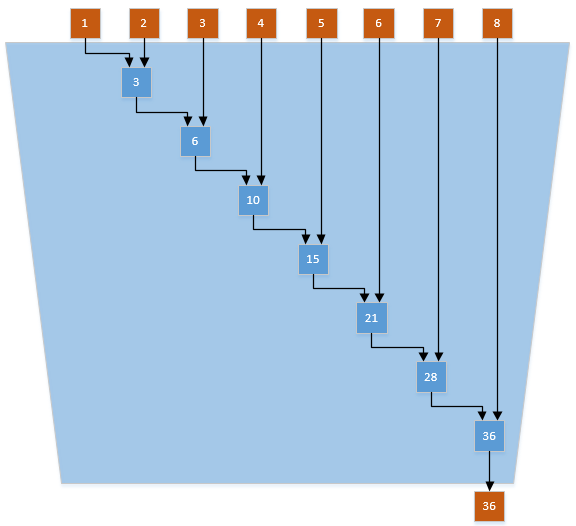
\includegraphics[width=0.5\textwidth]{figs/algorithm/reduce_serial.PNG}}
	\caption{Visual representation of the serial implementation of the reduction algorithm. The orange squares represent data elements, while the blue represent $\oplus$ operations}
	\label{fig:reduce_serial}
\end{figure}

Each operator operation in the serial implementation is data depend, which creates a chain of dependencies. The serial reduction is common for single core system and is commonly implemented using a loop. The step and work complexity for the serial reduction is $\mathcal{O}(n)$. Because of the data dependency in the serial reduction its operations cannot execute in parallel. A parallel reduction based on a binary tree is seen on \cref{fig:reduce_parallel}, here several of the operations can executed in parallel, thereby reducing the step complexity of the algorithm. 

\begin{figure}[ht]
	\centering
	\fbox{
		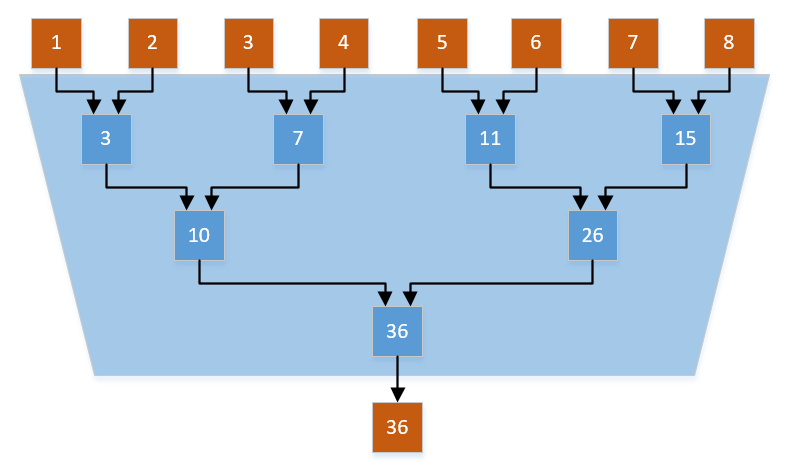
\includegraphics[width=0.6\textwidth]{figs/algorithm/reduce_parallel.png}}
	\caption{Visual representation of the parallel implementation of the reduction algorithm. The orange squares represent data elements, while the blue represent $\oplus$ operations}
	\label{fig:reduce_parallel}
\end{figure}

The binary tree parallel reduction has a work complexity of $\mathcal{O}(n)$ and a step complexity of $\mathcal{O}(log ~ n)$, thereby step efficient. 
The amount of data dependency is reduced, making it more suitable for parallel execution. A simple CUDA implementation of a reduction algorithm is seen in appendix \cref{ch:app_code_examples} in listing \ref{lst:reduce_kernel}. A fully working reduction can be found in \cite{exercises}. It should be noted that this example is not optimized, but is merely to show how a CUDA implementation looks. The shown implementation uses global memory and will only work on arrays smaller than the maximum threads per block. A way of making the reduce work on an arbitrary array size, is by combining multiple reductions as presented on \cref{fig:al_reduce_combine}:

\begin{figure}[ht]
	\centering
	\fbox{
		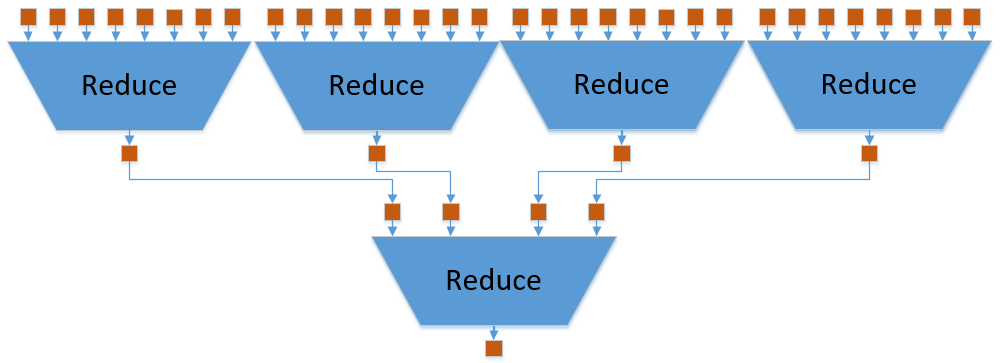
\includegraphics[width=0.9\textwidth]{figs/algorithm/reduce_combine.png}}
	\caption{Reduction using a reductions per thread block}
	\label{fig:al_reduce_combine}
\end{figure}

The combination of reductions enables reduction of both arbitrary array sizes and different array dimensions. Shared memory used by each  can also further optimize the reduction implementation.

The reduction algorithm is used in many application within parallel computing. An example of use is in Monte Carlo simulation, used in e.g. finance, computer graphics, image processing, where averages and variances of large arrays is needed.

	
	\section{Scan}
	\label{sec:al_scan}
	A common, simple and highly used building bloc for parallel algorithms is all-prefix-sum denoted scan. Scan calculates all partial reductions of a set, as defined by Blelloch \cite{BlellochTR90} in \cref{def:al_blelloch_scan}.

\begin{definition}
\label{def:al_blelloch_scan}
\textit{The scan operation takes a binary associative operator $\oplus$, and an ordered set of n elements}
\begin{center}
$[a_0,a_1,...,a_{n-1}],$
\end{center}
\textit{and returns the ordered set}
\begin{center}
$[a_0, (a_0 \oplus a_1),...,{a_0 \oplus a_1 \oplus ... \oplus a_{a_n-1}}].$
\end{center}
\end{definition} 

The scan, like the reduction in \cref{sec:al_reduction}, is using the binary associative operator, and can therefore be used for e.g. addition or multiplication. There is distinguished between two types of scan, the exclusive scan also named prescan and the inclusive scan also just named scan. The inclusive scan is defined as \cref{def:al_blelloch_scan} where as exclusive scan is defined accordingly to Blelloch \cite{BlellochTR90} as \cref{def:al_blelloch_prescan}:

\begin{definition}
	\label{def:al_blelloch_prescan}
	\textit{The prescan operation takes a binary associative operator $\oplus$ with identity I, and an ordered set of n elements}
	\begin{center}
		$[a_0,a_1,...,a_{n-1}],$
	\end{center}
	\textit{and returns the ordered set}
	\begin{center}
		$[I,a_0, (a_0 \oplus a_1),...,{a_0 \oplus a_1 \oplus ... \oplus a_{a_n-2}}].$
	\end{center}
\end{definition} 

Both types of scan can be acquired from the other by using shifting. They are both used in different applications benefiting from there differences. Blelloch \cite{BlellochTR90} also describes the scan as a good example of an algorithm that seems inherently sequential, but for which there is an efficient parallel implementation. \Cref{fig:scan_serial} show a visual representation of the common serial implementation of the scan.  

\begin{figure}[ht]
	\centering
	\fbox{
		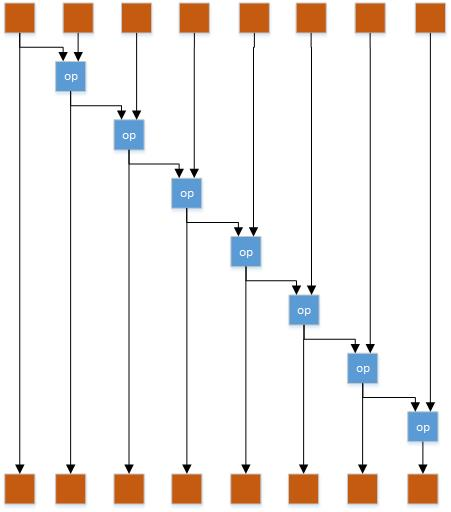
\includegraphics[width=0.4\textwidth]{figs/algorithm/scan_serial.jpg}}
	\caption{TBD}
	\label{fig:scan_serial}
\end{figure}

The algorithm looks a lot like the serial reduction on \cref{fig:reduce_serial}, but cannot be paralleled the same way because of the more strict chain of dependencies. Like the serial reduction the serial scan has a work and step complexity of O(n). The next two subsections will describe two different parallel implementations of the scan algorithm.
	
		\subsection{Hillis/Steele Scan}
		\label{sec:al_scan_hillis_steele}
		One way of implementing a parallel scan is with the algorithm developed by Hillis and Steele \cite{Hillis:1986:DPA:7902.7903}. This implementation is also called the naive parallel scan, because of its work inefficiency. A visual representation of the algorithm is show in \cref{fig:scan_hillis_steele}. 

\begin{figure}[ht]
	\centering
	\fbox{
		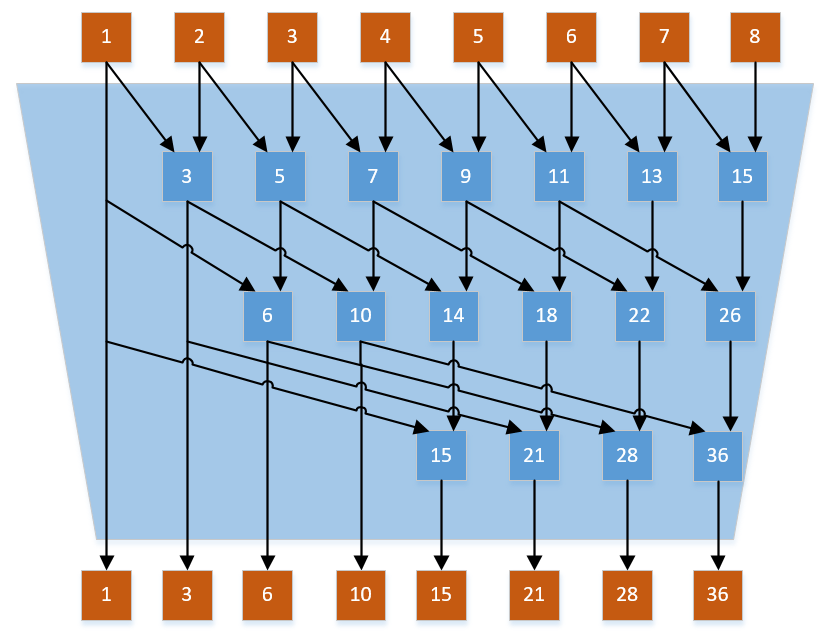
\includegraphics[width=0.6\textwidth]{figs/algorithm/scan_hillis_steele.png}}
	\caption{Naive inclusive scan developed by Hillis and Steele}
	\label{fig:scan_hillis_steele}
\end{figure}

The algorithm iterates through $log~n$ steps, where $n$ is the number of array elements to sum. At each step each element is combined through the binary associative operator with its right $ 2^k $ neighbor, where $k$ is the step depth starting at zero. The Hillis/Steele is natively a inclusive scan but can be implemented as an exclusive scan e.g. by shifting. The step complexity of the Hillis/Steele scan is $\mathcal{O}(log~n)$, thereby step efficient. The work complexity on the other hand is $\mathcal{O}(n~ log~n)$, making it work inefficient. The algorithm assumes that there is as many processors in the system as there is data elements to be combined, this is not always the case. For small array sizes the Hillis/Steele scan is efficient, as it will keep the processors busy, and create the result in few steps. A kernel implementation of the Hillis/Steele scan can be found in \cref{ch:app_code_examples} in listing \ref{lst:hillis_steele_scan_kernel}. A fully working example can be found in \cite{exercises}.
		
		\subsection{Blelloch Scan}
		\label{sec:al_scan_blelloch}
		Another implementation of the scan is with the algorithm developed by Blelloch \cite{BlellochTR90}. The Blelloch scan is based on a balanced tree
		
		\subsection{Blocking Scan}
		\label{sec:al_scan_blocking}
		As with the reduction, individual scans can be combined into larger scans. Doing this, small individual scans can run in individual thread blocks, thereby enabling the usage of shared memory. The visual representation in \cref{fig:scan_blocking} shows a 1D implementation strategy for scanning of arrays larger than maximum block thread sizes.

\begin{figure}[ht]
	\centering
	\fbox{
		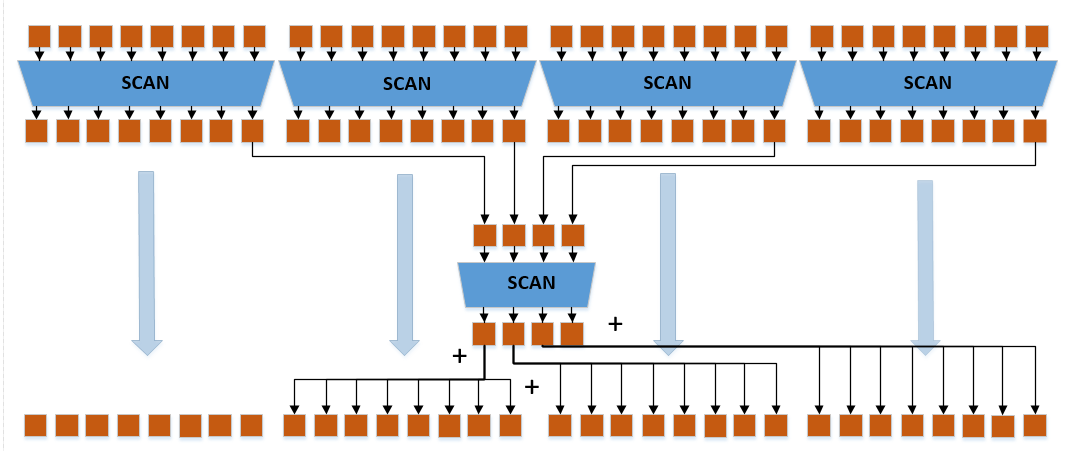
\includegraphics[width=0.9\textwidth]{figs/algorithm/scan_blocking.png}}
	\caption{Scanning of arbitrary array sizes, where individual thread block, run independent scan, later combined to the final array}
	\label{fig:scan_blocking}
\end{figure}

The idea is to divide the array into smaller arrays each with a maximum array size of the maximum threads per block. Then a individual scan is perform on each of the individual arrays. The reduction sum of each array is collected into a new array, on which a scan is performed, creating all the partial sums of the input array. The partial sums are summed with there respective individual array, thereby creating the total scanned output. 
	
	\section{Histogram}
	\label{sec:al_histogram}
	Histograms are used in many applications, often data analysis, and are probability density function approximations for given data arrays. A histogram is an algorithm that counts the number of observations within specified data range sections called bins. A histogram consists of bins which individually defines a range of values within the entire data value range. The output of a histogram is made by counting the number of data values that fall into each bins range. A formal definition with a concrete example of the histogram is seen in \cref{def:al_histogram}.

\begin{definition}
	\label{def:al_histogram}
	\textit{The histogram operation takes an ordered set of m elements, representing the bins}
	\begin{center}
		$[b_0,b_1,...,b_{m-1}],$
	\end{center}
	\textit{and an ordered set of n data elements}
	\begin{center}
		$[a_0,a_1,...,a_{n-1}],$
	\end{center}
	\textit{and returns the ordered set}
	\begin{center}
		$[\sum_{i=0}^{n-1}(1\{ a_i \leq b_0 \}),\sum_{i=0}^{n-1}(1\{b_0 \leq a_i \leq b_1\}),...,\sum_{i=0}^{n-1}(1\{b_{m-2} \leq a_i \leq b_{m-1}\})],$
	\end{center}
	\textit{where $1\{a\leq b\}$ is the indicator function returning one if $a\leq b$ else zero.}
\end{definition}
\begin{example}
	With the bin array
		\begin{center}
		$[3,6,9],$
	\end{center}
	and the data array 
		\begin{center}
		$[1,4,1,7,1,5,3,12],$
	\end{center}
	the return is
		\begin{center}
		$[4,2,2].$
	\end{center}
\end{example}

Histograms are used in a variety of applications including, data analysis, image processing, data representation and data mining. Several parallel algorithms and application also use the histogram functionality including the radix sort presented in \cref{sec:al_sort_radix}. The task of implementing a serial histogram is rather trivial, and the pseudocode of such implementation is seen in listing \ref{lst:histogram_serial}.

\begin{lstlisting}[language=C,caption={TBD},label=lst:histogram_serial]
for( int i = 0; i < BIN_COUNT; i++){
	result[i] = 0}; 
for( int i = 0; i < DATA_COUNT; i++){ 
	result[COMPUTE_BIN(data[i])]++}; 
\end{lstlisting}

Firstly, each of the result array locations is instantiated to zero Secondly, the data input array is loop for each element, and the resulting bin result array locations is calculated and incremented. The serial histogram has the work and step complexity $\mathcal{O}(n)$. The serial implementation is easy implemented for single threaded purposes, while a parallel implementation is quite difficult. 

           
	
		\subsection{Naive Histogram}
		\label{sec:al_hist_naive}
		Their are several different implementation strategies for parallel histogram algorithms. One possible strategy, often called the naive implementation, work by spawning a thread for each data element. Each thread, associated with one data element, computes the correct bin and increments the corresponding output array element. Without concurrency control race conditions will arise, because two or more threads may try to increment the same output array element at the same time. The concurrency control for the naive histogram implementation is the atomicAdd function.

\begin{lstlisting}[language=C,caption={Pseudo code for naive implementation of histogram using atomics},label=lst:histogram_atomicadd]
__global__ void naive_histo_kernel(int *d_bins, const int *d_in, const int BIN_COUNT)
{
	int myId = threadIdx.x;
	int myItem = d_in[myId];
	int myBin = COMPUTE_BIN[myItem];
	atomicAdd(&(d_bins[myBin]), 1);
}
\end{lstlisting}

The code for a simple naive histogram implementation in CUDA is seen in listing \ref{lst:histogram_atomicadd}. The implementation defines the thread id which is used to find the associated input array element. The corresponding bin is calculated using an application specific function, here defined as COMPUTE\_BIN. The CUDA specific atomicAdd is used to increment the correct bin, as it prevents race conditions. The naive parallel histogram has a work complexity of $\mathcal{O}(n)$, as one thread is allocated each data element. The step complexity is harder to define, as it varies based on the data input an number of bins. The step complexity depends on the dependency chain course by the concurrency control, as the atomicAdd will serialize the access to the output array element. When there are few data elements per bin then contention is low and the execution is fast, whereas many data elements per bin will increase the contention making execution slow. 

The naive solution presented above has limited scalability as the atomic operation will limit the parallelism, as the number of simultaneously working thread is limited to the number of bins. Besides the naive strategy there are two strategies that are commonly used for parallel histograms, as presented in the study in \cite{MilicHistogram}. We denote the two strategies histogram by privatisation and histogram by sort. These two strategies will be explained in the following sections.
		
		\subsection{Histogram by Privatization}
		\label{sec:al_hist_privatization}
		
The histogram by privatization is a optimized version of the naive strategy. The shortcomings of the naive strategy is the limited scalability caused by the thread contention in the atomic operation. The histogram by privatization tries to limit this shortcoming by decomposing the input data into smaller batches. An individually histogram is calculated by a thread block for each batch. The individually histograms is combined to created the final histogram. Doing the histogram calculation this way will limit the thread contention as the maximum amount of waiting threads are reduced from the input array size to amount of threads per block.
The individually thread blocks will besides the limited contention also benefit from the possible use of shared memory. Each thread block will create its own shared histogram, using shared memory and shared atomics. The usage of both shared memory and shared atomics will increase the performance. When each thread in a block is finished the private histogram is added to the global final histogram. For this addition there are two possible solution. Each solution is illustrated in \cref{fig:hist_privat}. 

\begin{figure}[ht]
	\centering
	\begin{subfigure}{0.9\textwidth}
		\centering
		\fbox{
			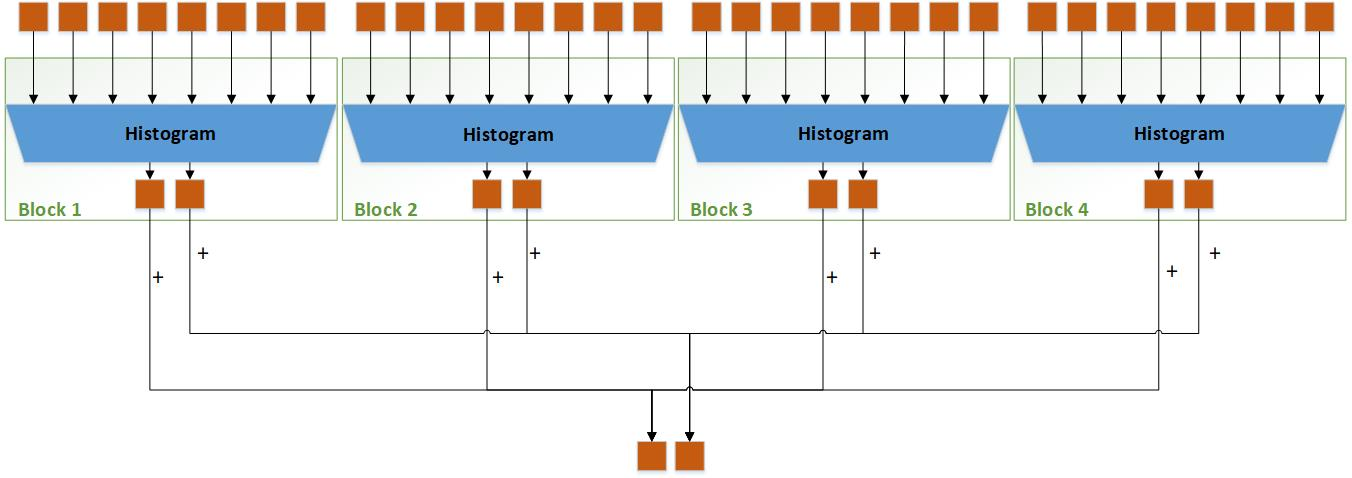
\includegraphics[width=0.9\textwidth]{figs/algorithm/hist_privat_atomic.jpg}}
		\caption{TBD}
		\label{fig:hist_privat_atomic}
	\end{subfigure}
	\begin{subfigure}{.9\textwidth}
		\centering
		\fbox{
			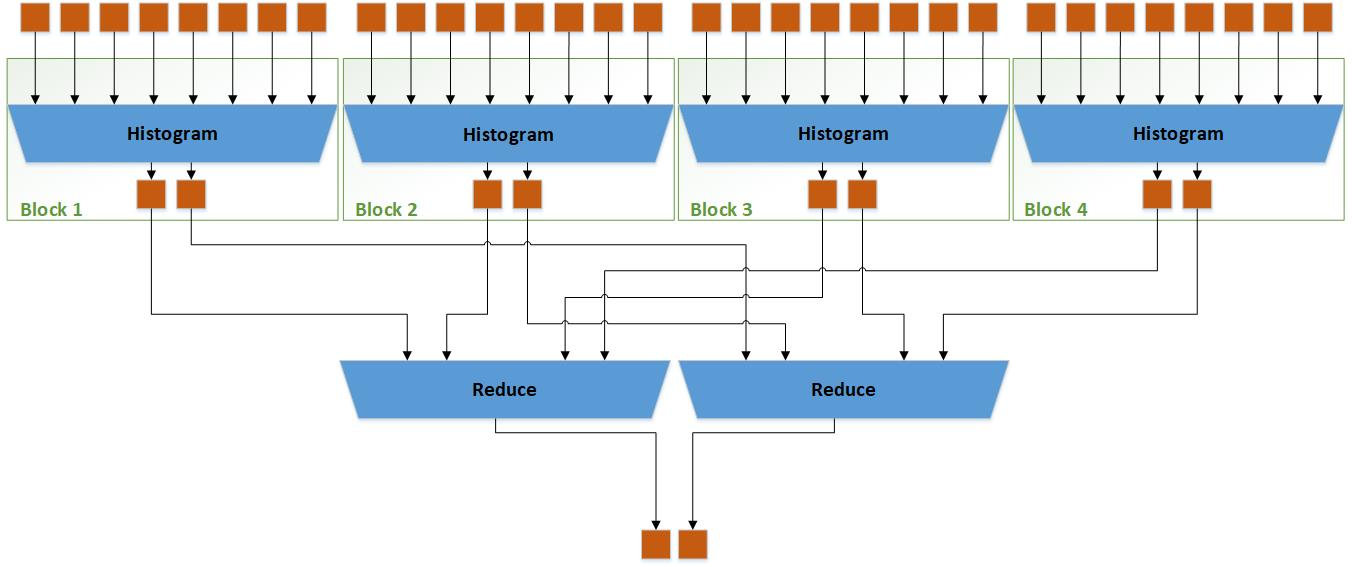
\includegraphics[width=0.9\textwidth]{figs/algorithm/hist_privat_reduce.jpg}}
		\caption{TBD}
		\label{fig:hist_privat_reduce}
	\end{subfigure}
	\caption{TBD}
	\label{fig:hist_privat}
\end{figure} 

The first addition solution as seen in \cref{fig:hist_privat_atomic} is to add the private histogram to the global histogram with atomics. As the naive and private  implementations the effectiveness of this solution is limited by the thread contention. The other solution, presented in \cref{fig:hist_privat_reduce} is to use the reduction algorithm from \cref{sec:al_reduction}. The reduction algorithm would be a good alternative to the atomic version, to avoid contention,  when there are many private histograms.       
		
		\subsection{Histogram by Sort}
		\label{sec:al_hist_sort}
		The final histogram strategy is the histogram by sort, and is unlike the histogram by privatization very different from the naive strategy. The idea behind the histogram by sort is to first sort the input array, and then calculates the histogram based number of element within the given bin widths. The histogram by sort eliminates the thread contention which was the limiting factor in the naive and privatization strategies, but may introduce a lot of overhead caused by the sort algorithm. An visual example of the histogram by sort is seen in \cref{fig:hist_sort}. 

\begin{figure}[ht]
	\centering
	\fbox{
		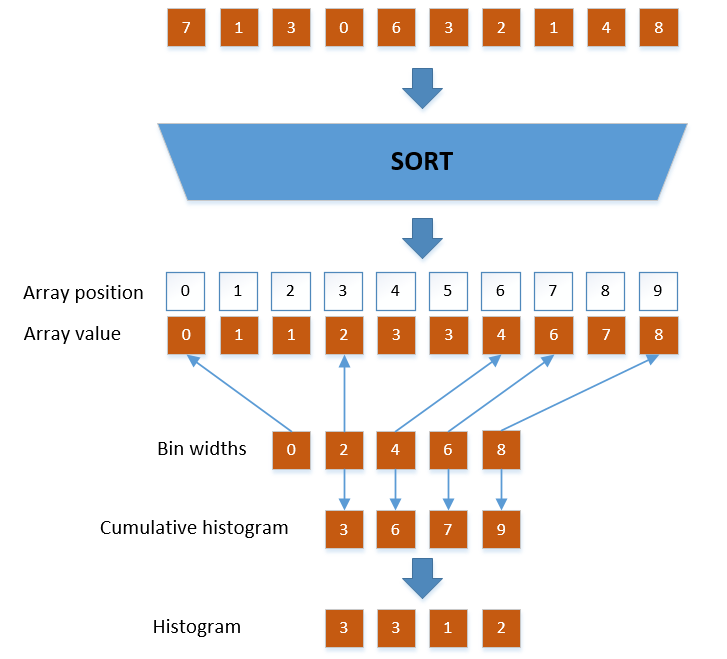
\includegraphics[width=0.5\textwidth]{figs/algorithm/hist_sort.png}}
	\caption{Histogram by sort}
	\label{fig:hist_sort}
\end{figure} 

Firstly, the input array is sorted using a parallel sorting algorithm, like the ones presented in \cref{sec:al_sort}. After the sorting the bin widths, predefined to the histogram function call, are used to find the upper bounds of array positions. The upper bound is found by writing the highest array position, of a specific bin width value to a new array, as seen in \cref{fig:hist_sort}. This upper bound array is the cumulative histogram, and the final histogram is then found by subtracting the left neighbour element from each element in the array. 
The histogram by sort has a high overhead because of the sorting, but may be better than the histogram by privatization, when the number of input element is high, the number of bins is high or when the input data is not uniformly distributed. In all of those cases the histogram by privatization will be limited by the serialization cause by the atomic operations. These are also the conclusions in the histogram study by \cite{MilicHistogram} and a final note is that parallel histogram strategies are highly application specific.
	
	\section{Sort}
	\label{sec:al_sort}
	The ability to sort an array is a important in programming, both for serial and parallel applications. Sorting and array mean to order the element in a specific way, this could be both numerical or lexicographical. This section will only focus on examples and sorting of numerical minimum to maximum sorting. A formal definition of the numerical minimum to maximum sort is seen in   

\begin{definition}
	\label{def:al_sort}
	\textit{The sort operation takes an unordered set of n elements}
	\begin{center}
		$[a_0,a_1,...,a_{n-1}],$
	\end{center}
	\textit{and returns permutation}
	\begin{center}
		$sgn([a_0,a_1,...,a_{n-1}])$
	\end{center}
\end{definition}
\begin{example}
	With the input array
	\begin{center}
		$[3,6,9,1,2,6,2,3],$
	\end{center}
	the return of the sort is
	\begin{center}
		$[1,2,2,3,3,6,6,9].$
	\end{center}
\end{example}

There are many way of implementing a sorting algorithm both in the serial and in the parallel context. Many factors a present when choosing a sorting algorithm for an application. For the serial implementations examples of sorting algorithm is Quicksort, Merge sort, Heapsort and Bubble sort. The average work complexity of the serial sorting algorithm is $\mathcal{O}(n~log~n)$, so a  
	
		\subsection{Odd-Even Sort}
		\label{sec:al_sort_odd}
		One of the simplest parallel sorting algorithms is odd-even sort also know as odd-even transposition sort and brick sort. It is a comparison sort and can be seen as the parallel version of the simple serial bubble sort. The odd-even sort consists of two phases a odd and an even. In each phase each odd or even index array pair is compared and swapped if necessary. An visual representation of the odd-even sort is seen in \cref{fig:sort_odd_even}.

\begin{figure}[ht]
	\centering
	\fbox{
		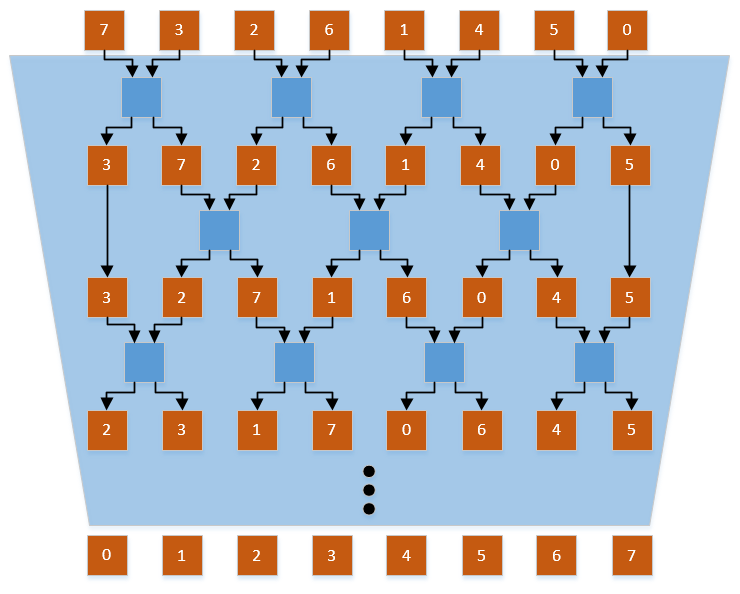
\includegraphics[width=0.5\textwidth]{figs/algorithm/sort_odd_even.png}}
	\caption{Odd-even sort, orange blocks are data elements, and blue blocks are compare-and-swap operations}
	\label{fig:sort_odd_even}
\end{figure}  

The odd-even sort have a worst-case step complexity of $\mathcal{O}(n)$ as the maximum number of array position an element can move is $n$. The worst case work complexity is $\mathcal{O}(n^2)$ as $\mathcal{O}(n)$ operations is carried out in $\mathcal{O}(n)$ steps. The odd-even sort is step efficient when compared to serial versions, but other parallel sorting algorithms are more efficient.   
		
		\subsection{Merge Sort}
		\label{sec:al_sort_merge}
		The merge sort is a divided and conquer comparison sort, having both a serial and parallel version. The idea behind the merge sort, is to first divide the input data into 1 element subsets. Then each pair of subsets are merged by sort, creating a new smaller set of sorted subsets. The merging step is carried out until the number of subsets reach 1, representing the final sorted output data. A visual representation of the merge sort is seen in \cref{fig:sort_merge}.

\begin{figure}[ht]
	\centering
	\fbox{
		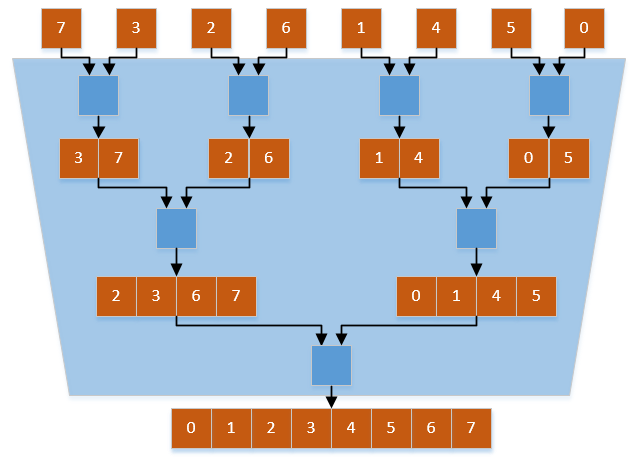
\includegraphics[width=0.5\textwidth]{figs/algorithm/sort_merge.png}}
	\caption{Merge sort}
	\label{fig:sort_merge}
\end{figure}  

The implementation of serial merge sort, is rather simple and can be done using recursion. That approach cannot be used for a parallel implementation, as load unbalance happens when few thread have to merge large arrays. Another approach is therefore necessary for a parallel merge sort. The parallel strategy consist of 3 stages; merge-per-thread, merge-per-block and merge-by-blocks. The first stage is carried out when there are a lot of small merges required. Each merge is allocated to one thread, thereby there are a lot of individual threads working in parallel utilizing the GPU. When the merges reach a size and number where only few threads will work a lot, the merge-per-block stage is enabled. In this stage each merge is carried out by multiple threads in a block. Each thread in a block is allocated one array element from one of the two merging arrays. Each thread then calculates the position of its element in the merged array, and writes the element to that position. This procedure is visual represented in \cref{fig:sort_merge_per_block}.     

\begin{figure}[ht]
	\centering
	\fbox{
		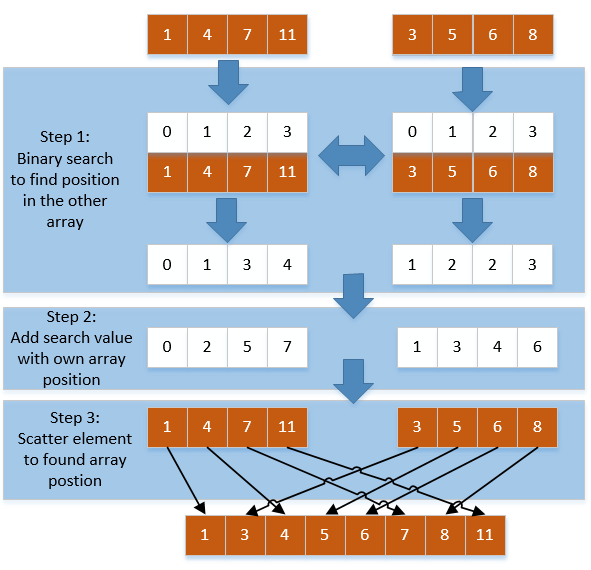
\includegraphics[width=0.5\textwidth]{figs/algorithm/sort_merge_per_block.png}}
	\caption{Merge sort merge-per-block}
	\label{fig:sort_merge_per_block}
\end{figure}  

First each thread uses binary search to find its elements position in the other merge array. Second that position is added with the elements own array position resulting in the array position in the final merged array. Third and last the thread writes the element to the merged array. The last stage of the merge sort is the merge-by-blocks. This stage is carried out when the merge arrays is to large for a single block, so when each element can not be assigned its own thread. The merging arrays are divided across thread blocks, thereby having multiple blocks working on the same merge. The merge sort, in its serial implementation, have a work and step complexity of $\mathcal{O}(n~log~n)$. In the parallel implementation, there is a work complexity of $\mathcal{O}(n~log~n)$ and a step complexity of $\mathcal{O}(log^2~n)$, thereby working better than both the serial implementation and the odd-even sort.  
	
		\subsection{Radix Sort}
		\label{sec:al_sort_radix}
		The Radix sort is another example of a sorting algorithm having both a serial and an parallel implementation. The Radix sort can be considered brute force, and is a non-comparison algorithm. The idea behind the radix sort is to sort each elements by its elements bits. The way the radix sort works can be divided into three steps as seen in \cref{tab:radix}.

\begin{center}
	\fbox{
		\begin{tabular}{p{40pt} p{220pt}}
			\textbf{Step 1} & Start with LSB \\
			\textbf{Step 2} & Split input into 2 sets based on bit values, otherwise preserve order \\
			\textbf{Step 3} & Move to next MSB, repeat
		\end{tabular}
	}
	\captionof{table}{Steps of Radix sort}
	\label{tab:radix}
\end{center} 

An example of the radix sort with the steps form \cref{tab:radix} is seen in \cref{fig:sort_radix}.

\begin{figure}[ht]
	\centering
	\fbox{
		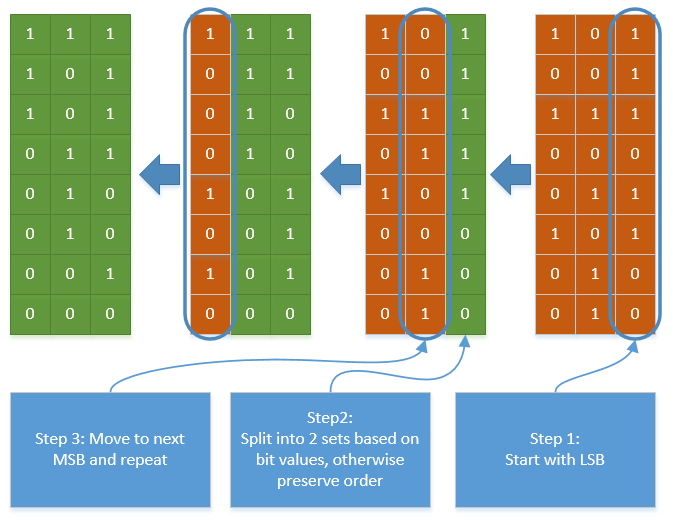
\includegraphics[width=0.7\textwidth]{figs/algorithm/sort_radix.png}}
	\caption{Radix sort}
	\label{fig:sort_radix}
\end{figure}  

The Radix sort have a work complexity of $\mathcal{O}(kn)$ where k is the number og bits, and a step complexity of $\mathcal{O}(k)$. The radix sort is therefore highly depended on the number of bits in the numbers to sort. The radix will also often have a better work and step complexity, when compared with other sorting algorithms. The radix sort is a good example of an algorithm that is not very efficient in serial, but rather efficient in parallel, because of the high parallelization. The implementation of the radix sort is explained in the \cref{sec:exercise4}.   


		\subsection{Quick Sort}
		\label{sec:al_sor_quick}
		Quicksort is a divide and conquer comparison sorting algorithm, and has both a serial and parallel implementation. Serial quicksort is one of the most frequently used sorting algorithms, because of its simple implementation and high efficiency. The quicksort work by choosing a pivot, and then sorting the elements based on the pivot, creating new subsets. Each new subset is then sorted by pivot again, resulting in the creation of the final array. The quicksort can be described using the steps seen in \cref{tab:quicksort}.

\begin{center}
	\fbox{
		\begin{tabular}{p{40pt} p{220pt}}
			\textbf{Step 1} & Choose pivot element\\
			\textbf{Step 2} & Compare all elements with pivot \\
			\textbf{Step 3} & Split into 3 array; less than pivot, equal to pivot and greater than pivot \\
			\textbf{Step 4} & Recurse on each array
		\end{tabular}
	}
	\captionof{table}{Steps of Quicksort}
	\label{tab:quicksort}
\end{center} 

The first step is to choose the pivot, for which there are many strategies e.g. first element, last element, random element or median element. The choice of the pivot is the limiting factor of the quicksort, choosing the wrong pivot, increases the step and work complexity to $\mathcal{O}(n)$ and $\mathcal{O}(n^2)$ respectively. Then the pivot is chosen right the quicksort has a step complexity of $\mathcal{O}(log ~ n)$ and a work complexity of $\mathcal{O}(n~log~n)$, proving the choose of pivot is important. The second step is to compare all the elements with the pivot. The third step is to create three arrays, one containing all the numbers below the pivot, one with all numbers equal to the pivot and one with all numbers above the pivot. This is called the 3-way quicksort. The fourth and final step is to recurse on the above and below array, calling the quicksort again. An example of the quicksort, using last element as pivot is seen in \cref{fig:sort_quicksort}.

\begin{figure}[ht]
	\centering
	\fbox{
		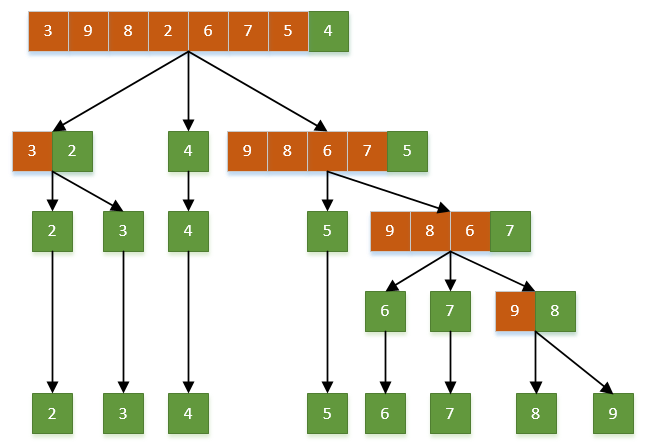
\includegraphics[width=0.7\textwidth]{figs/algorithm/sort_quicksort.png}}
	\caption{Example of the Quicksort, using last element pivot.}
	\label{fig:sort_quicksort}
\end{figure}  

One can implement the quicksort without recursion, but that is rather complicated, and is not as efficient as calling the quicksort with recursion. Not all languages and architectures support recursion, and this functionality was also first incorporated into the CUDA programming model in the 3.1 Toolkit \cite{cuda_3.1}.        

	\section{Compact}
	\label{sec-compact}
	The term compact in computing refers to an input set of potentially many inputs where only a subset of those inputs are used to make a computation.
In other words compact filters an input space into a subset.
Using compact before doing computations is both more computation and memory efficient, if only some inputs of the entire data space are of interest.

More formally the compact algorithm takes an input and computes a new output based on a predicate.
The input is a set \textit{S} with \textit{n} inputs, where 
\begin{gather}
	S=\{s_{0}, s_{1}, s_{2}, ... , s_{n}|n\in \mathbb{R}\}
\end{gather}
The predicate is a function that inputs an \textit{S}, $f_{P}(S)$, and returns \textit{true} or \textit{false} for each $s_n$.
The returned output, $O\in S$, contains all input elements where the predicate is \textit{true}. 
Since not all predicates are necessarily \textit{true} means that the output is $O\subseteq S$.
Furthermore, \textit{O} can have a sparse or dense representation.
For a sparse output each $f_{P}(S)\equiv \mathtt{true}$ is assigned to its same position in \textit{O}, while $f_{P}(S)\equiv \mathtt{false}$ are assigned as \textit{none} (an empty element or some sort of \textit{null} value).
On the other hand, for a dense output $\mathtt{O}=\{s\ |\ s\in f_{P}(S)\equiv \mathtt{true}\}$.

As an example say we have the following input and predicate function
\begin{align}
	       S &= \{0, 8, 26, 12, 24, 50\}, \\
	f_{P}(S) &= \{s\ \mathtt{mod}\ 4 = 0\ |\ s\in S\}
\end{align}
The predicate function thus results in
\begin{gather}
	f_{P}(S)=\{\mathtt{true}, \mathtt{true}, \mathtt{false}, \mathtt{true}, \mathtt{true}, \mathtt{false}\}
\end{gather}
Then the output of such a compact operation results in
\begin{align}
	O_{sparse} &= \{0, 8, \mathtt{none}, 12, 24, \mathtt{none}\}\\
	O_{dense} &= \{0, 8, 12, 24\}
\end{align}

In parallel it is more efficient to use the dense compact algorithm since this results in only spawning threads that actually have a computational task to do.
Implementing the dense compact algorithm in parallel is done by using scatter adresses.
Scattering addresses is done by using the scatter pattern where each input is scattered to another place in memory as described in \autoref{sec-scatter}.
For example if the predicate function for some \textit{S} returns the following set
\begin{gather}
	f_{P}(S_{rand}) = \{\mathtt{true}, \mathtt{false}, \mathtt{false}, \mathtt{true}, \mathtt{true}, \mathtt{false}, \mathtt{true}, \mathtt{false}\}
\end{gather}
the desirable indexes in the scatter output is the set $\{0, -, -, 1, 2, -, 3, -\}$, where "-" are "don't care".
To compute the scatter adresses can be done by doing an exclusive scan as described in \autoref{sec:al_scan}.
First the result of $f_{P}(S)$ is translated into zeros and ones using a such that
\begin{gather}
	f_{P}(S_{rand})_{new} = \{1, 0, 0, 1, 1, 0, 1, 0\}
\end{gather}
Finally the scatter addresses are computed by doing an exclusive sum scan on $f_{P}(S_{rand})_{new}$ which gives
\begin{gather}
	\{0, 1, 1, 1, 2, 3, 3, 4\}
\end{gather}
In this way it known to which indexes each input element should be scattered to in the output element.
Note that the actual inputs are only those where the predicate function is evaluated to true.
The compact algorithm is summarized into following steps:
\begin{center}
	\fbox{
	\begin{tabular}{p{40pt} p{220pt}}
			\textbf{Step 1} & Use predicate on input elements, $f_{P}(S)$, and translate the results into zeros and ones \\
			\textbf{Step 2} & Do an exclusive sum scan on the zeros and ones array, $f_{P}(S_{rand})_{new}$, from step 1. The output is scatter addresses for the compacted array.\\
			\textbf{Step 3} & Scatter the input array into the output array using the scatter addresses.
	\end{tabular}
	\label{alg-compact}
	}
	\captionof{table}{Steps to compact}
\end{center}

Implementation - compare sparse vs dense
%TODO: make implementation of both
	
	\section{Allocate}
	\label{sec-allocate}
	The allocate algorithm generalizes the compact algorithm described in \autoref{sec-compact}.
Before reading this section it is advised to read \autoref{sec-compact}.
The compact algorithm generates a single output for each input that is evaluated as \textit{true}, according to a given predicate, and generates no output elements for input values which are evaluated to \textit{false}.
The allocate algorithm can compute a number of output elements dynamically for each input element.
The main difference is that the transformation function of $f_{P}(S)_{new}$ does not translate to only zeros and ones, but into \textit{n} needed allocation requests.
The idea is illustrated in \autoref{fig:allocate} and as can be seen the predicate function here ranges with values from zero to three as opposed only zero and one as in the compact algorithm.
\begin{figure}[ht]
	\centering
	\fbox{
		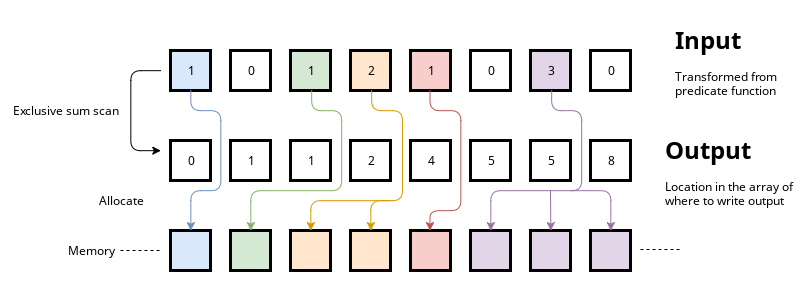
\includegraphics[width=0.85\textwidth]{figs/algorithm/allocate.png}
	}
	\caption{Example of allocate}
	\label{fig:allocate}
\end{figure}
The steps in the allocate algorithm are the same as described in \autoref{alg-compact}.
Usage of this kind of algorithm is very use case specific, but in general if it is desired to do a compact operation on varying sizes of objects the this algorithm makes it possible to achieve this.

%TODO: maybe small code example but ommit if no time
	
\chapter{Optimization}
\label{ch-opti-intro}
As previously mentioned, when parallelizing a task, the goal is to achieve a higher throughput of the task performed by the program. While parallelizing could be assumed to directly improve the throughput, one has to take different things into account, one of the most important, how well is the program optimized for the task it performs. The goal when optimizing a program is to make the best or most effective use of the data, calculations, and resources for the task to be performed. Specifically for optimization of CUDA programs, we will look at three different aspects, general optimization, memory access optimization and threat divergence influence on performance. These three aspects will be discussed in the following sections, where the focus will be on non-application specific optimization, providing strategies for optimization which can be applied to a broad range of programs. 

\section{General Optimization}
\label{sec-general-opti}
When performing general optimization of CUDA codes, threre are different levels of optimization.
\begin{enumerate}
	\item Picking a good algorithm
	\item Basic principles for efficiency
	\item Architecture specific detailed optimization
	\item Micro optimization at instruction level
\end{enumerate}

\section{Optimization of Memory Access}
\label{sec-opti-memory}
One of the most important things when optimizing CUDA code is optimizing the memory access done by the kernel which is being executed. The CUDA GPU memory model, which is described in depth in \cref{sec-hw-memory-model}, contains five levels of memory going from smallest and fastest to largest and slowest, \texttt{Registers}, \texttt{Shared Memory}, \texttt{Level 1 Cache}, \texttt{Level 2 Cache} and \texttt{Global Memory}. While all of these should be kept in mind, while optimizing a CUDA program, it can be seen in \cref{sec-pm-memory} in the chapter describing the programming model, that when programming, there is only four type of memory to be concerned with, \texttt{Host Memory}, \text{Global Memory}, \text{Shared Memory} and \texttt{Local Memory}.\\
To optimize global memory access another concept needs to be introduced, which is coalesced memory. Where the indication for the memory here is that coalesced memory is memory, which is closely related, thereby placed next to each other when looking at the address space of the memory. When threads in each streaming multiprocessor are divided into Warps (SIMT Units), as discussed in \cref{sec-hw-warps-threads}, the Warp, as they are SIMT, are also in charge of issuing memory reads and writes. The Warp here attempts to issue global memory access into as few transactions as possible to minimize DRAM bandwidth. This, in turn, means that to optimize memory access, we have to have threads access memory, which is in the address space is next to each other. In turn, this also increases performance as the Warp will not have to issue reads or writes for a single thread out of the 32 threads contained within a Warp.\\

\begin{figure}[ht]
	\centering
	\fbox{
		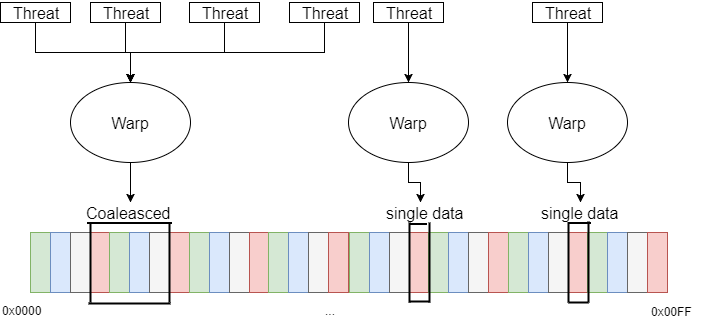
\includegraphics[width=0.9\textwidth]{figs/opti/coalesed_memory.png}
	}
	\caption{Example of coalesced memory access vs random memory access, where other threads are idle while the warp is accessing memory.}
	\label{fig:coalesced_memory}
\end{figure}

\Cref{fig:coalesced_memory} show how multiple threads being in the same warp, accesses coalesced memory. The reason for coalesced memory being important is that single data access is often just as expensive in time as it is to access larger pieces of data. This is because memory is only read in chunks, which correlates to a single read being able to supply multiple threads with data or a single threat with a large amount of data of which there is no guarantee that it uses all of.\\

However, it is very difficult to avoid all random memory access, which is where our memory model become important, as different levels of memory are available for use. Instead of using the slower \texttt{Global memory}, \texttt{Shared memory} can be used for the random memory access. This can be accomplished by using shared memory as a buffer. As shared memory is faster, these memory accesses will also be performed faster. As an example of the optimization gain, we can take a look at two different reduce kernels, one which does direct access to global memory, and one which makes use of shared memory. The code for the reduce kernel without any optimization can be found in listing \ref{lst:reduce_kernel}.\\

Using the kernel to sum 2048 elements, a runtime could be measured. To get a more precise measurement, the kernel was run a thousand times on the same elements, thus calculation an average runtime of 0.971 ms. To optimize the before mentioned reduce kernel, shared memory was used internally in the kernel, the code can be seen in listing \ref{lst:reduce_shared}.

\begin{lstlisting}[language=C,caption={TBD},label=lst:reduce_shared]
__global__ void reduce_kernel_shared(unsigned *in, unsigned *out) 
{
	auto id = blockDim.y * blockDim.x * blockIdx.x + threadIdx.y * blockDim.x + threadIdx.x;
	__shared__ int sdata[K/2];
	sdata[id] = in[id * 2] + in[id * 2 + 1];
	for(size_t i = 1 ; i< K/2; i *= 2) 
	{
		if (id % (2 * i) == 0)
			sdata[id] += sdata[id + i];
		__syncthreads();
	}
	if (id == 0) 
		out[0] = sdata[0];
}
\end{lstlisting}

Performing the same measurements as before, an average runtime of 0.831 ms was calculated. And while this performance difference may not seem very significant it is still an improvement, and running the kernel on a larger array then 2048 elements, might give even further improvements.\\

In the end, memory optimization is some of the best ways to gain improvements in performance with CUDA programs, however like most optimization is difficult, and often gives less performance per hour spend than other things, such as picking a better algorithm as described in \cref{sec-general-opti}. That being said, the core terms explained in this section, being coalesced memory and shared memory, can for some algorithms be fairly simple to implement.

\section{Thread Divergence}
\label{sec-thread-div}
Whereas memory access optimization can be related to warps, thread divergence is purely related to how threads are executed within a warp. As described in \cref{sec-hw-warps-threads} a warp is a Single Instruction Multiple Threads unit, which can only run a single instruction set at a given time on all threads, which means every time a branching is encountered, some threads might stale while others instruction set is being executed. An example of branch divergence could be based on a simple switch case within a kernel. For branch divergence, only the case itself is important which can be seen in listing \ref{lst:branch_div}.\\

\begin{lstlisting}[language=C,caption={Dividing threads into warps, using modulus operator},label=lst:branch_div]
switch(thread_id % 2)
{
	case 0:
		sdata[id]--;
	case 1:
		sdata[id]++;
}
\end{lstlisting} 

So the kernel in listing \ref{lst:branch_div} would be a simple kernel which accesses some global memory, and if the index of the shared memory is even, its decremented if it is odd its increment. To fully understand how this example would be influenced by branch divergence, it is important to understand how the thread IDs are assigned, as in this, and most other cases, it is the ID which would be used to determine to branch. As described in \cref{sec-pm-threads} threads receive both an X, Y and Z id within their block, and their block receives an X, Y, and Z index as well. From these, a global ID can be constructed which is normally what is used when writing CUDA programs. When threads are assigned to Warps, this happens by first assigning the X IDs, then the Y IDs and last the Z IDs. Thereby if a block is created with X dimension of 32 and a Y dimension of 32, as Warps contain 32 threads we will have that all threads within the Warp have the same Y ID and X ID ranging from 0 to 31. A visualization of this can be seen in \cref{fig:id_warp}.\\

\begin{figure}[ht]
	\centering
	\fbox{
		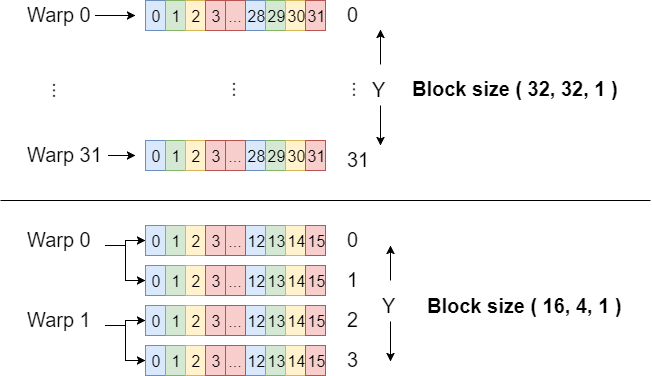
\includegraphics[width=0.9\textwidth]{figs/opti/ID_warp.png}
	}
	\caption{Threads ID's inclusion in Warps.}
	\label{fig:id_warp}
\end{figure}

Based on the before mentioned kernel being executed with a block size of (32, 32 1), and using the knowledge of how thread ID's are assigned, it can then be determined that every second thread within a Warp will take the first case, and every other will take the second case. Had this been a computation which far out weighted that of the switch case and calculating the global index, the execution time would be approaching two times that which would be expected if there had been no such thing as Warps.\\

Therefore, while thread divergence may not always be a huge factor when it comes to slowdowns, it is worth noting that thread divergence within Warps clearly affects the execution time of a kernel. Which means that there are cases where it might be worth optimizing threat divergence. The approach here is to arrange the branches or data different, such that more threats within a Warp will take the same route through the code of the kernel. For the code listed in listing \ref{lst:branch_div} this could have been achieved by having another data arrangement and then changing the code to what can be seen in listing \ref{lst:branch_div2}.

\begin{lstlisting}[language=C,caption={Creating a better arrangement of threads to allign with warps},label=lst:branch_div2]
switch(thread_id / 32)
{
	case 0:
		sdata[id]--;
	case 1:
		sdata[id]++;
}
\end{lstlisting} 

And while it may not be possible for all code to do such a rearrangement, similar optimization might be worth considering if optimizing performance critical applications with a lot of branching.

\chapter{Applications}
\label{ch-app}
There are multiple applications that parallel algorithms and patterns can be applied to.
Some application examples are given in the following section.
	
	\section{Sparse Matrix/Dense Vector Multiplication}
	\label{sec-matrix}
	Lesson 4 and 6.1
	
	\section{Graph}
	\label{sec-graph}
	\begin{itemize}
	\item Traversal of graphs
	\item Depth first traversal
	\item Breadth first traversal
	\item In parallel
	\item Work complexity
	\item Optimizing runtime for graph traversal (lesson 6.2) very detailed and complex to describe in writing. Beware
\end{itemize}

Lesson 6.1
	
	\section{Exercises}
	\label{sec:exercises}
	This section contains a detailed description along with solution methods, to each of the six exercises available in the Udacity online course Intro to Parallel Programming \cite{udacity:parallel}. The code used to solve the exercises can be found on GitHub\cite{exercises}.
	
		\subsection{Exercise 1}
		\label{sec:exercise1}
		This exercise focuses on conversion from a color image to a black and white image.
Color images, are often represented by the intensity of red, green and blue also called RGB values.
The value zero represents an absent color and 255 saturated color, so if all RGB values are zero, the the pixel is black, and if all values are 255, then pixel is white.
In the exercise it is recommended to do the conversion with the following formula instead of simply averaging the RGB values.
This is because the human does not perceive colors equally.
\begin{align*}
I = 0.229\cdot R + 0.587\cdot G + 0.114\cdot B
\end{align*} 
In \cuda{} a pixel can be represented by a struct \textit{uchar4} that holds four members, x (red), y (green), z (blue) and w (alpha: component that describes the transparency).
The \textit{w} component is not relevant when converting to gray scale.

\noindent The result of the conversion can be seen in \autoref{fig:ex1} and the source code in \cite{exercises}.
\begin{figure}[ht]
	\centering
	\begin{subfigure}{.5\textwidth}
		\centering
		\fbox{
			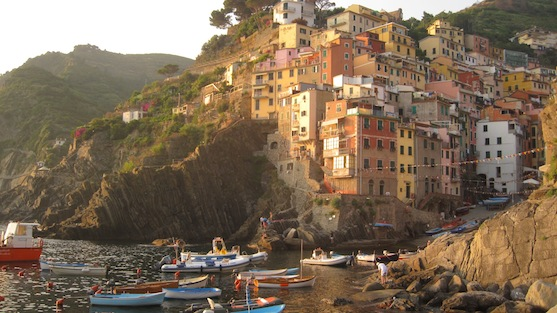
\includegraphics[width=0.7\textwidth]{figs/exercises/ex2/cinque_terre_small.jpg}
		}
		\caption{Before}
		\label{fig:ex1-before}
	\end{subfigure}%
	\begin{subfigure}{.5\textwidth}
		\centering
		\fbox{
			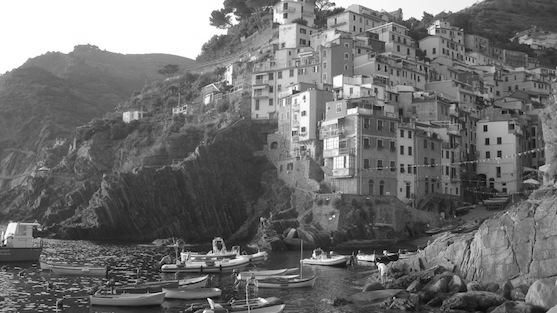
\includegraphics[width=0.7\textwidth]{figs/exercises/ex1/HW1_output.png}
		}
		\caption{After}
		\label{fig:ex1-after}
	\end{subfigure}
	\caption{Picture before and after conversion to gray scale}
	\label{fig:ex1}
\end{figure}
The following steps are performed to solve the exercise.
\begin{enumerate}
	\item[\textbf{Step 0}]
	\textit{Write a kernel that converts the pixels from RGB to gray scale}.
	This can be done by generating a unique id for each thread, depending on the blockIdx, blockDim and threadIdx in both x and y which determines the pixel to convert.
	When the "global" thread id has been extracted, the pixel RGB value is simply converted using the formula above.
	\item[\textbf{Step 1}]
	\textit{Launch the kernel with a reasonable block and grid size}.
	As the picture is relatively large, it could be beneficial to create the block size as $32\times32$ (1024 is the maximum number of threads in a block) threads and then a grid of blocks depending on the number of rows and columns of the image.
\end{enumerate}
		
		\subsection{Exercise 2}
		\label{sec:exercise2}
		Exercise 2 addresses implementing a parallel algorithm for blurring images.
The original image, which is used in the exercise is presented on \cref{fig:ex2-before}.
The image blurring process can be done in different ways, however for this excise, the \textit{neighbor weighted average} technique is used.
It is done, by taking the pixel representation of an image, as illustrated on \cref{fig:ex2}, and for each pixel, multiply the selected pixel and its surrounding pixels with predefined weighted values:

\begin{align*}
\omega_{avg} &= (\omega_1 \cdot p_1) + (\omega_2 \cdot p_2) + ... + (\omega_N \cdot p_N) 
\end{align*} 

Once these weighted pixel values are calcdaulated, they are added together to define the new blurred pixel value for the center pixel. 
By performing this operation onto every pixel of the original image, the resulted blurred image is seen on \cref{fig:ex2-after}.
The averaging through neighbor weighted average is expressed naturally using a parallel stencil operation as described in \cref{sec-stencil}.
The weighing filter can have various appearances, however the one used in the exercise is shown on \cref{fig:ex2} marked with blue colors.

\begin{figure}[ht]
	\centering
	\begin{subfigure}{.5\textwidth}
		\centering
		\fbox{
			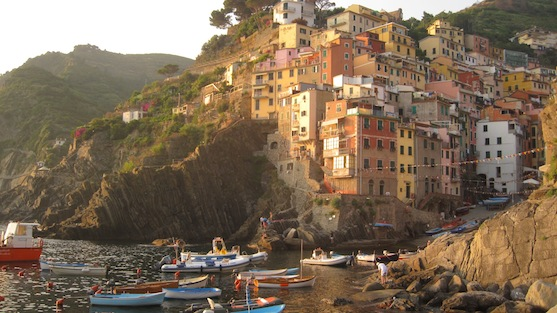
\includegraphics[width=0.8\textwidth]{figs/exercises/ex2/cinque_terre_small.jpg}
		}
		\caption{Before}
		\label{fig:ex2-before}
	\end{subfigure}%
	\begin{subfigure}{.5\textwidth}
		\centering
		\fbox{
			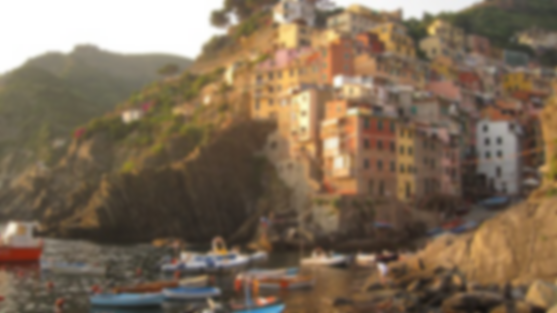
\includegraphics[width=0.8\textwidth]{figs/exercises/ex2/HW2_output.png}
		}
		\caption{After}
		\label{fig:ex2-after}
	\end{subfigure}
	\caption{Picture before and after blur effect is added}
	\label{fig:ex4}
\end{figure}

\begin{figure}[ht]
	\centering
	\fbox{
		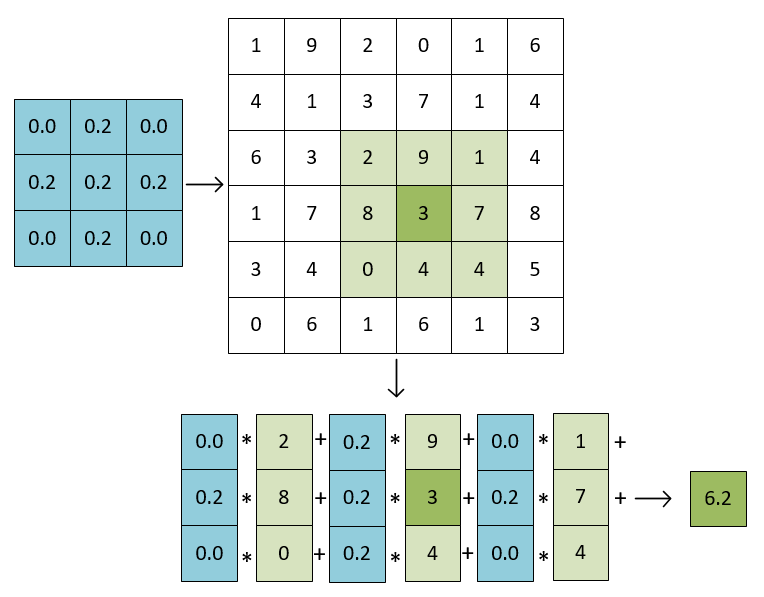
\includegraphics[width=0.8\textwidth]{figs/exercises/ex2/hw2.PNG}
	}
	\caption{TBD}
	\label{fig:ex2}
\end{figure}

Prior to the blurring itself, the colored image is separated in the three color channels red, green \& blue, in order to store each color contiguously instead of having it interleaved, which is done to simplify the remaining exercise.
\\\\
The exercise is separated into four steps, which are presented below, to see the entire source code of the exercise, see \cite{exercises}.

\begin{enumerate}
	\item[\textbf{Step 1}] First write a kernel to separate a colored image into R, G \& B channels.

	\item[\textbf{Step 2}] Next step is to write the blurring kernel, running through all pixels and perform the blurring filtering described earlier.
	Here care must be taken to clamp neighboring values to be within the bounds of the image, to ensure no reads of neighboring pixel values lying outside of the image is performed. 
	

	\item[\textbf{Step 3}] The third step is to allocate memory for the filter used.
	This should be done using \texttt{cudaMalloc} as described in \cref{sec-pm-memory} and ensuring nothing goes wrong by using \texttt{checkCudaErrors}.

	\item[\textbf{Step 4}] Last step is to compute the optimum grid size based on the image size and the block size.
	Finally, the three blurred channels are combined to create the blurred final image.
\end{enumerate}


		
		\subsection{Exercise 3}
		\label{sec:exercise3}
		This exercise focuses on histogram equalization, which is a method of contrast adjustment in images. Many images are taken in the High Dynamic Range (HDR) format, enabling devices to capture a wider range og colors. When we display images we can only show them in the 8 bit range meaning, when displaying a HDR image using float values, a lot of details are lost when mapped. When mapped directly an image consisting of many dark colors in a narrow range, may resulting in an image as seen on \cref{fig:ex3-before}.
Therefor when mapping an image from the float range to the 8 bit range, a histogram equalization may be necessary. In histogram equalization the pixels are scales so the whole range of an image is used equally, as represented on \cref{fig:histogram_eq}. 

\begin{figure}[ht]
	\centering
	\begin{subfigure}{.5\textwidth}
		\centering
		\includegraphics[width=0.5\textwidth]{figs/exercises/ex3/memorial_raw.png}
		\caption{Before}
		\label{fig:ex3-before}
	\end{subfigure}%
	\begin{subfigure}{.5\textwidth}
		\centering
		\includegraphics[width=0.5\textwidth]{figs/exercises/ex3/memorial_gold.png}
		\caption{After}
		\label{fig:ex3-after}
	\end{subfigure}
	\caption{Picture before and after histogram equalization}
	\label{fig:ex3}
\end{figure}  

\begin{figure}[ht]
	\centering
	\includegraphics[width=0.5\textwidth]{figs/exercises/ex3/histogram_eq.png}
	\caption{Histograms of an image before and after equalization \cite{wiki:hist_eq}}	\label{fig:histogram_eq}
\end{figure}  

Instead of working with all the channels in the RGB space, the image is converted to YUV space, as only one channel needs to be equalized, namely the Chrominance-Luminance. The task of the exercise is to calculate the cumulative distribution of the luminance channel. This can be done through 4 steps, as presented below.
\begin{enumerate}
	\item[\textbf{Step 1}]
	Find the minimum and maximum value in the luminance channel. This can be done through two different reduction algorithms, having the binary associative operator maximum or max and minimum or min respectively. One should also consider the size of the luminance array, as it is larger than the  thread block size.  
	\item[\textbf{Step 2}]
	Find the range of the luminance values, which is the difference between the minimum and maximum values calculated in step 1. 
	\item[\textbf{Step 3}]
	Calculate a histogram of the values in the luminance array. the number of pixels in each image pixel range needs to be calculated so the image histogram can be found. The way the bin for the histogram is chosen is through the equation \cref{eq:bin}.
	
	\begin{equation}
	\label{eq:bin}
		bin = \frac{(lum[i]-lumMin)}{lumRange}*numBins
	\end{equation}
	
	When running the histogram in parallel, one should consider the race condition scenario where multiple threads may try to write to the same address. This scatter operation, can be solved, using e.g. atomics, but more clever and efficient methods may be used. 
	\item[\textbf{Step 4}]
	Lastly the cumulative histogram is calculated using a scan operation on the histogram. The scan should be an exclusive scan, so the scan algorithm by Blelloch may be a good choice.  
\end{enumerate}  
		
		\subsection{Exercise 4}
		\label{sec:exercise4}
		This exercise focuses on red eye removal from a picture (in this case, the picture on \autoref{fig:ex4-before}).
The specified sequence of steps is to start out by computing a score for each pixel that estimates the likelihood of that pixel belonging to a read eye (higher score is more likely).
The score is known as normalized cross-correlation and is expressed naturally as a stencil operation.
This score has already been computed in the exercise and the next step is therefore to sort these scores in ascending order (likelihood) effectively.
The final step is to reduce the redness of the highest scoring pixels and this can be performed using simple map operations.
As stencil and map operations have already been worked on in previous exercises, the focus of this exercise is to perform the sorting efficiently.
The result of the red eye removal can be seen in \autoref{fig:ex4-after}.
\begin{figure}[ht]
	\centering
	\begin{subfigure}{.5\textwidth}
		\centering
		\fbox{
			\includegraphics[width=0.4\textwidth]{figs/exercises/ex4/red_eye_effect_5.jpg}
		}
		\caption{Before}
		\label{fig:ex4-before}
	\end{subfigure}%
	\begin{subfigure}{.5\textwidth}
		\centering
		\fbox{
			\includegraphics[width=0.4\textwidth]{figs/exercises/ex4/HW4_output.png}
		}
		\caption{After}
		\label{fig:ex4-after}
	\end{subfigure}
	\caption{Picture before and after red eye removal}
	\label{fig:ex4}
\end{figure}

\noindent The actual exercise is to implement a parallel radix sort as described in \autoref{sec:al_sort_radix}.
To compute the sort, a lot of work has to be done (the actual source code can be seen in \cite{exercises}.)
The following sequence of techniques are performed for every bit of the values to sort (32bit values in this exercise).
The steps are visualized in \autoref{fig:ex4-radix-sort}.
\begin{enumerate}
	\item[\textbf{Step 1}]
	An exclusive prefix sum scan is performed over a "vector" of predicates (ones or zeros).
	This is done for both the zeros and ones to sort.
	For the ones to sort, the predicate is true if the bit is one and false if it is zero, and the other way around (inverted) for the zeros to sort.
	It is used to determine the scattering offset address.
	Because the number of elements to sort is larger than the maximum number of threads in a thread block, the kernel must be executed using multiple thread blocks.
	As it is only possible to synchronize threads within a block, the resulting scan is actually a segmented scan, which is not the desired operation in this context.
	\item[\textbf{Step 2}]
	Because of the segmented scan operation, it is necessary to store the highest scattering offset address, and use this later to convert the segmented scan to a regular scan. 
	\item[\textbf{Step 3}]
	An exclusive prefix sum scan is performed on the elements stored from \textbf{Step1} to generate the offset value which should be added to the elements of the segmented scan.
	\item[\textbf{Step 4}]
	A histogram of the number of ones and zeros is generated.
	\item[\textbf{Step 5}]
	An exclusive prefix sum scan is performed over the histogram.
	This is to generate the scattering offset to where the zeros and ones should start in the resulting vector.
	\item[\textbf{Step 6}]
	In the last step, the results of the precious steps are used to generate the resulting vector of sorted ones and zeros.
	The result from \textbf{Step 4} determines the start offset for zeros (0) and ones (7).	
	The value on index "blockId" from the result in \textbf{Step 2} is added to all elements in each block of the segmented scan from \textbf{Step 0}.
	When this is performed for both zeros and ones, the resulting vector contains the sorted zeros and ones.
\end{enumerate}
\begin{figure}[ht]
	\centering
	\fbox{
		\includegraphics[width=1.0\textwidth]{figs/programming-model/ex4-radix-sort.pdf}
	}
	\caption{Exercise 4 radix sort implementation}
	\label{fig:ex4-radix-sort}
\end{figure}
%For every bit, starting a LSB, a histogram of the number of occurrences of each digit (0 or 1)
%Exclusive prefix sum scan of histogram
%predicate kernel (return vector with 1 for all ones and a vector with 1 for all zeros)
%Exclusive prefix sum scan of predicates, exclusive prefix sum scan of incr values and add kernel at the end
%move kernel, move to position if predicate is one
%swap input and output (out of order sort)
		
		\subsection{Exercise 5}
		\label{sec:exercise5}
		The task itself in exercise 5 is quite simple, one simply has to code a histogram kernel. The main program provided, generates 10.240.000 random distributed numbers, with a mean ~500, and a standard divination of 100. Thus the goal is to create a histogram kernel, to create a histogram of the values, using principles for CUDA optimization to perform the task as fast as possible.\\

The first approach to solve this is, to simply create a histogram kernel, which can do the histogram, and ignore optimization at all.

\begin{lstlisting}[language=C,caption={Histogram kernel},label=lst:histogram_kernel]
void yourHisto(unsigned int* const vals, //INPUT
	unsigned int* const histo,      //OUPUT
	int numVals) {
	unsigned idx = blockIdx.x * blockDim.x + threadIdx.x;
	if (idx >= numVals )
		return;
	atomicAdd(&(histo[vals[idx]]), 1);
}
\end{lstlisting}

Running the above histogram kernel on the 10.240.000 random numbers takes, 4.0 ms on a computer, with a Nvidia GTX 980TI graphic card.\\ 
Looking at the code, it is, however, easy to identify some possible optimization steps. Applying the more memory levels, in this case, shared memory should significantly lower the run time of the kernel.\\
 
 \begin{lstlisting}[language=C,caption={Introducing shared memory into the histogram kernel},label=lst:histogram_kernel2]
void yourHisto(unsigned int* const vals, //INPUT
	unsigned int* const histo,      //OUPUT
	int numVals) {
	__shared__ unsigned ar[1024];
	unsigned idx = blockIdx.x * blockDim.x + threadIdx.x;
	for(int i = 0 ; i < 1000 ; ++i)
		atomicAdd(&(ar[vals[idx + i * 10240]]), 1);
	__syncthreads();
	atomicAdd(&histo[threadIdx.x], ar[threadIdx.x]);
}
 \end{lstlisting}
 
 As can be seen in listing \ref{lst:histogram_kernel2}, a shared memory block is introduced, allowing the threads within a block to access it. While the kernel still uses atomic to write to this memory, it should still be significantly faster. To ensure that the thread block is finished before the shared memory is added to the global, \texttt{syncthreads} is used. Each thread is also performing 1000 more operations, in that an internal loop is introduced. Using an offset in each iteration ensures that threads within a thread block, which is on the same iteration, still accesses memory coalesced\\
Running the kernel again, now reduces the run time to 2.4 ms, on the same computer as before. further tweaking the number of iterations in the internal loop yields far better results. The best configuration, with the specific hardware, is ~100 iterations per thread in the internal loop, lowering the runtime of the kernel to 1.1 ms.\\
		
		\subsection{Exercise 6}
		\label{sec:exercise6}
		In this exercise the task at hands is to clone one image into another, using seamless image cloning as can be seen in \cref{fig:cloning}. The given code for this exercise is very sparse, providing only the calls to a function \texttt{your\_blend} which is empty of functionality, but does contain some description of the work which has to be done.\\

To do this a few new concept is used such as double buffering, which uses two buffers, one which is used to perform computations on, from which the result is written into the second buffer. In the next iteration, the roles of the buffers are then swapped, and the same computations are done again. Other things include creating a mask from the source image to determine border and interior pixels on the polar bear image, and transposing RGB values, to separate into array of channel values instead of array of RGB values.\\

Last, to do the "merging" part of the cloning process solves a Poisson equation to determine how the image is to be blended. To solve the Poisson equation the exerciser gives a method, based on Jacobi Iterations, which provides the following formula for computing the value of a pixel:

\begin{align*}
I_{k+1} &= \frac{A + B + C}{D}
\end{align*} 

To determine A, B, C and D the concept neighbors is used, which is the index of the pixels besides the given pixel. Neighbors can only be with on or within the border of the mask created. Using this, A, B, C, D is as follows:

\begin{itemize}
	\item A is sum of the pixels interior neighbors in the buffer
	\item B is the sum of the pixels border neighbors in the target image
	\item C is difference between the pixel and its neighbors on the source image
	\item D is number of neighbors.
\end{itemize}

This computation is done for each of the channels which in the image, thus for R, G and B., In the end, the three individual channels are combined to make a whole image.

\begin{figure}[ht]
	\centering
	\fbox{
		\includegraphics[width=0.9\textwidth]{figs/exercises/ex6/merged.png}
	}
	\caption{The source image of a polar bear is to be cloned onto a destination picture of an swimming pool.}
	\label{fig:cloning}
\end{figure}

There are several steps involved in implementing this task, here the task is divided into work, corresponding to the kernels, being called in the solution:
\begin{enumerate}
	\item[\textbf{Step 1}]
	The first step is to create the mask, based on the source image, to determine the border and interior pixels of the source image. The source image contains either some RGB value or else (255, 255, 255) for everything that is not supposed to be cloned into the destination. These values can then be used for creating the mask inside a kernel.
	\item[\textbf{Step 2}]
	Transpose both the source and destination image from RGB values to separate arrays for each color channel.
	\item[\textbf{Step 3}]
	Assign the initial value for the guess to solving the Poisson equation to each of the two buffers. The initial value used is the one from the source image.
	\item[\textbf{Step 4}]
	Run the Jacobi iterations 800 times as assign by the exercise. This will give an approximation that is converging towards the correct solution. The Jacobi kernel performs the before mentioned equation in each iteration, based on the input buffer, and assigns the values to the output buffer. After each iteration, the two buffers are swapped.
	\item[\textbf{Step 5}]
	Lastly after 800 iterations the output buffer for each color channel is used to construct a combined image, which is the completed result of the seamless image clone.


\end{enumerate}
		
\chapter{CUDA Libraries}
\label{ch-libraries}
This section exemplifies how CUDA can be utilized and invoked in different environments.
Furthermore this section describes some libraries for parallel programs that exploit CUDA.
There are are many libraries for CUDA so only a few selected will be concerned in this section.

	\section{Thrust}
	\label{sec-thrust}
	Until now this report has described many parallel patterns, algorithms and applications.
Common for all are that they can be very cumbersome to implement and are prone to many  errors which are difficult to find such as wrong memory allocation, off-by-one errors, complex and unreadable source code, high algorithm complexity and deep understanding of CUDA and the underlying architecture.
\\\\
Thrust is a C++ library which enables programming of high performance applications with minimal programming efforts.
It is based on the Standard Template Library (STL) and gives a rich collection of data parallel primitives such as scan, sort and reduce.
Since the desired computation is described in a high abstraction level, Thrust will try to optimize and select the most efficient implementation.

Thrust is basically built upon three building blocks which are vectors, algorithms and iterators.
There are two types of vectors in Thrust: \textit{host\_vector} and \textit{device\_vector}.
Host vectors are stored in host memory while device vectors are stored in device memory.
This is makes allocation and copying between host and device relatively straight forward.
An example of this is seen in \autoref{lst:thrust-vec}.
\begin{lstlisting}[language=C,caption={Vectors in Thrust},label=lst:thrust-vec]
#include <thrust/host_vector.h> 
#include <thrust/device_vector.h> 
int main(void) { 
	thrust::host_vector<int> H(4); 
	...// Initialize H
	thrust::device_vector<int> D = H; 
	...// Modify D directly
	return 0;
}
\end{lstlisting}
There are many benefits of using Thrust vectors.
For instance the vectors can be resized and copying between host and device is straightforward by the overloaded "="-operator.
Furthermore, both host and device vectors are deleted and the memory is freed once the function returns.
Thrust also gives useful functions for copying and initializing data on the host and device.
Examples of such functions are \textit{thrust::fill}, \textit{thrust::sequence} and \textit{thrust::copy}.
It is still possible to extract raw CUDA device pointers from Thrust vectors

Thrust enables easy usage of parallel communication patterns and algorithms as described in \autoref{ch-patterns} and \autoref{ch:algorithms}.
Following are some examples of such patterns and algorithms which are supported in Thrust:
\begin{itemizeSmall}
	\item thrust::reduce
	\item thrust::inclusive\_scan
	\item thrust::exclusive\_scan
	\item thrust::sort
	\item thrust::sort\_by\_key
	\item thrust::stable\_sort
\end{itemizeSmall}
For instance an exclusive scan is seen in \autoref{lst:thrust-scan}

\begin{lstlisting}[language=C,caption={Exclusive scan in Thrust},label=lst:thrust-scan]
#include <thrust/scan.h> 
...
int data[6] = {1, 0, 2, 2, 1, 3}; 
thrust::exclusive_scan(data, data + 6, data); // data becomes {0, 1, 1, 3, 5, 6}
...
\end{lstlisting}
This simplifies a lot TODO REF TO CODE EXAMPLE HERE IF TIME.

Using the Thrust library also enables the usage of fairly complex iterators.
Some of the iterators in Thrust are:
\begin{description}
	\item[Constant iterator] The \textit{constant\_iterator} returns the same value whenever it is accessed.
	\item[Counting iterator] The \textit{counting\_iterator} increments its value by one with respect to the initialization value.
	\item[Permutation iterator] The \textit{make\_permutation\_iterator} allows to fuse for example gather and scatter operations into a single iterator. This is a rather complex subject so it will not be discussed in depth in this report.
	\item[Zip iterator] The \textit{zip\_iterator} takes multiple input sequences and returns a sequence of tuples. It is rather useful if for instance one would like to iterate over two distinct data types in a single loop.
\end{description}
All operators in Thrust are accessed like arrays.
\\\\
This was only an introduction to Thrust and which features there are that can ease CUDA application development, where many of the core CUDA details are abstracted away.
This of course makes it easier and faster to prototype GPU applications, but at the cost of total control of the GPU.
For more info of Thrust see \url{http://docs.nvidia.com/cuda/thrust/index.html}. (should this be a ref in stead?)
	
	\section{PyCUDA}
	\label{sec-pycuda}
	PyCUDA enables execution of Python code on a CUDA device from a Python-script.
PyCUDA wraps all CUDA functionality and enables execution of kernels and copying data between the host and the device.
A major advantage of using PyCUDA in Python scripts is that execution times are potentially sped up.

Typical Python structures and libraries such as the popular \textit{numpy} library can be used in conjunction with PyCUDA, which is a huge benefit for researchers and developers working in this high level scripting language but would still like to be able to boost their algorithm performance.

Nevertheless, using PyCUDA has some CUDA knowledge preliminaries.
Kernels are written as C++ code, which are parsed to the device.
This means that the user of PyCUDA needs to know how to write such kernels.
There are a lot of features and details which will not be explained here.
This section is merely here such that the reader is aware of that CUDA utilization exists in Python.
For more information of PyCUDA and how it can be used please see \url{https://documen.tician.de/pycuda/}.
	
	\section{CUDA in MATLAB}
	\label{sec-matlab}
	MATLAB is a scripting language which is very widely used among engineers, data scientists, researchers and more.
It is often used for algorithm development, data analysis, data visualization and mathematical modeling.
MATLAB also supports GPU computing, where functions can be executed on the GPU, and more specifically it provides mechanisms of how to interface to a CUDA GPU.

Using MATLAB with a GPU can very speed up many algorithms, especially those who compute on large data sets such as the pixels of an image.

The MATLAB profiler can be used to identify computationally heavy sections in the script. 
Such sections indicate that GPU acceleration might be useful.
The easiest way to utilize the GPU via MATLAB is by converting an input array to a GPU array with the \textit{gpuArray(input)} function call in MATLAB.
It also possible to invoke a CUDA kernel directly from MATLAB for example by using the function shown in \autoref{lst:matlab}.
\begin{lstlisting}[language=matlab,caption={Invoking CUDA kernel in MATLAB},label=lst:matlab]
	kernel = parallel.gpu.CUDAKernel( 'someCUDAKernel.ptx', 'someCUDAKernel.cu' );
\end{lstlisting}
The \textit{.ptx} is needed for MATLAB when running the kernel and this file can be generated when compiling the \textit{.cu} file.
As can be seen CUDA can be utilized in multiple ways in MATLAB with relatively little effort.
For more information and full documentation on how to use a CUDA GPU in MATLAB see \url{www.mathworks.com/gpu}.
	
	\section{OpenCL}
	\label{sec-opencl}
	OpenCL (Open Computing Language) is a low-level API written in C/C++.
It is aimed for cross-platform computing and can be used for CPUs\footnote{Central Processing Unit} and GPUs, but also DSPs\footnote{Digital Signal Processor} and FPGAs\footnote{Field-programmable Gate Arrays}.

\begin{wrapfigure}{r}{0.31\textwidth}
	\centering
	\fbox{
		\includegraphics[width=0.3\textwidth]{figs/extra/opencl.png}
	}
	\caption{OpenCL concepts} 
	\label{fig:opencl}
\end{wrapfigure}

\noindent The core of OpenCL's programming model is that it views a computing system as a number computing devices that are attached to a host processor as shown in \autoref{fig:opencl}.
OpenCL enables parallel programming of heterogeneous systems and can be used to write and launch GPU kernels.
Many vendors such as Nvidia, AMD, Apple, Intel and Xilinx support OpenCL.
Using OpenCL enhances code portability, but at the expense of speed, since many optimizations are very platform dependent.

OpenCL's programming model reflects many of the same characteristics as in CUDA.
For instance, the memory model is very much alike where OpenCL's memory hierarchy defines four levels:
\begin{itemizeSmall}
	\item Global memory - shared by all devices with a high access latency.
	\item Read-only memory - smaller, low latency memory, where only the host CPU can write, while other computing devices only can read.
	\item Local memory - shared by a group of computing devices.
	\item Per-element private memory - corresponds to registers in each computing device.
\end{itemizeSmall}
Kernels are also written in a very similar way as in CUDA.
In general OpenCL programming resembles CUDA a lot.
Thus a transition from writing parallel programs in CUDA to OpenCL is somewhat straightforward since many of the concepts are the same.
	
	\section{Others}
	\label{sec-others}
	There exist libraries for CUDA and these constitute a large ecosystem of optimized algorithms which are designed for high performance.
Some of these libraries are:
\begin{itemizeSmall}
	\item [\textbf{cuBLAS}] Basic Linear Algebra Subroutines (BLAS) gives all needed functionalities to efficiently compute linear algebra problems.
	\item [\textbf{cuFFT}] API for doing Fast Fourier Transforms (FFT) routines.
	\item [\textbf{cuSparse}] BLAS-like routines, but optimized for sparse matrix formats.
	\item [\textbf{cuRAND}] Pseudo- and quasi-random number generation routines. This API is particular good and fast for filling arrays with numbers which are drawn from a particular distribution.
	\item [\textbf{NPP}] Nvidia Performance Primitives (NPP) is highly optimized for low-level image and video processing primitives. These include color conversion, image compression, image filters and more.
	\item [\textbf{CULA}] CULA is a set of GPU-accelerated linear algebra libraries which implements eigensolvers, matrix factorizations, matrix solvers and more.
\end{itemizeSmall}

\noindent A general advise is to use these libraries, if possible, instead of implementing a lot of already implemented functionalities from scratch.


% citation test
\cite{McCool2012}
\cite{udacity:parallel}

\bibliographystyle{plain}
\bibliography{bib}

\newpage
\appendix
\chapter{Reading Plan}
	?? TBD How should the reading plan be presented in the report?
\includepdf[pages=-]{figs/appendix/readingplan.pdf}

\end{document}
